% KOMA-Script Report-Template (A4, Times-ähnlich, deutscher Satzspiegel)
\documentclass[12pt,paper=a4,DIV=12,parskip=never,chapterprefix=false,headings=standardclasses]{scrreprt}

% --- Sprache & Encoding ---
\usepackage[T1]{fontenc}
\usepackage[utf8]{inputenc}
\usepackage[ngerman]{babel}

% --- Schrift (Times-ähnlich) & Mathematik, Mikrotypografie ---
\usepackage{newtxtext} % Textfont (Times-like, TeX Live)
\usepackage{newtxmath} % passende Matheschrift
\usepackage[final]{microtype}
\usepackage{caption}% stellt \captionsetup bereit

\usepackage{chngcntr}

% Schalter für die Abbildungsnummerierung
\newcommand{\FigureNumbersByChapter}{%
  \counterwithout{figure}{section}% alte Section-Kopplung lösen
  \counterwithin{figure}{chapter}% an Kapitel koppeln (reset auf 0)
}
\newcommand{\FigureNumbersBySection}{%
  \counterwithout{figure}{chapter}% alte Chapter-Kopplung lösen
  \counterwithin{figure}{section}% an Sektion koppeln (reset auf 0)
}

% --- Absatzlayout: Einzug, kein zusätzlicher Abstand ---
\setlength{\parindent}{1.5em}
\setlength{\parskip}{0pt}

% --- Seitenstil (unten Seitenzahl, schlicht) ---
\usepackage[headsepline=false,footsepline=false]{scrlayer-scrpage}
\clearpairofpagestyles
\cfoot{\pagemark}

\usepackage{float}
% --- Hyperlinks ---
\usepackage[hidelinks]{hyperref}
\usepackage{xurl}

% --- Bilder & Captions ---
\usepackage{graphicx}
\usepackage[font=small,labelfont=bf,labelsep=period]{caption}
\usepackage{subcaption}
\setcapindent{0pt}

\usepackage[most]{tcolorbox}
\usepackage{graphicx}
\usepackage{caption} % für \captionof

% --- Bequeme Referenzen (optional) ---
\usepackage[nameinlink,noabbrev]{cleveref}

\usepackage{siunitx}
\DeclareSIUnit{\ppm}{ppm}

\usepackage[most]{tcolorbox}
\usepackage{graphicx}
\usepackage{caption} % für \captionof

\usepackage{caption} % wichtig

\newtcolorbox{fullbox}[1]{%
  enhanced,
  breakable,
  colback=black!2,
  colframe=black,
  boxrule=0.4pt,
  left=6mm,right=6mm,top=4mm,bottom=4mm,
  title={\bfseries\Large #1},
  fonttitle=\bfseries\Large,
  coltitle=black,
  attach boxed title to top left={},
  boxed title style={colback=black!2,boxrule=0pt,left=0pt,right=0pt,top=0pt,bottom=2mm},
  before lower=\vfill,
  middle=0pt,
  segmentation style={draw=none} % <— trennt ohne Linie (auch bei page breaks)
}

\usepackage{amsmath}
%\numberwithin{figure}{chapter}
\FigureNumbersByChapter

\makeatletter
\renewcommand*{\tableofcontents}{%
  \begingroup
    \small      % Schriftgröße
    \sloppy     % vermeidet Zeilenumbrüche
    \chapter*{\contentsname}% <-- Überschrift zurück
    \@starttoc{toc}%
  \endgroup
}
\makeatother

% Kapitelname leer setzen:
\renewcaptionname{ngerman}{\chaptername}{}

% --- Titelseiten-Fonts: nicht fett ---
\setkomafont{title}{\normalfont\rmfamily\LARGE\mdseries}
\setkomafont{subtitle}{\normalfont\rmfamily\Large\mdseries}
\setkomafont{subject}{\normalfont\rmfamily\large\mdseries}
\setkomafont{author}{\normalfont\rmfamily\normalsize\mdseries}
\setkomafont{date}{\normalfont\rmfamily\normalsize\mdseries}
\setkomafont{titlehead}{\normalfont\rmfamily\mdseries}
\setkomafont{publishers}{\normalfont\rmfamily\mdseries}
\setkomafont{dedication}{\normalfont\rmfamily\mdseries}

% Kapitelüberschriften in VERSALIEN
\addtokomafont{chapter}{\MakeUppercase}

% Abschnittsüberschriften in VERSALIEN
\addtokomafont{section}{\MakeUppercase}

\IfFileExists{gitversion.tex}{\input{gitversion.tex}}{\def\gitversion{local-build}}
\usepackage{tikzpagenodes} % für sauberes Positionieren
\AddToHook{shipout/foreground}{%
  \begin{tikzpicture}[remember picture,overlay]
    \node[anchor=south, yshift=8mm] at (current page.south) {Version \gitversion};
  \end{tikzpicture}%
}

\begin{document}

% --- Deckblatt ---
\begin{titlepage}
\centering
\vspace*{-0.5cm}

\includegraphics[width=1.0\textwidth]{bilder/bilderKlima-0000.png}\\[1cm]

{\huge Eine kritische Überprüfung der Auswirkungen von Treibhausgasemissionen\\
auf das Klima in den Vereinigten Staaten\par}
\vfill
\begin{flushleft}
\Large
Climate Working Group\\
United States Department of Energy\\
July 23, 2025
\end{flushleft}
\vfill
\end{titlepage}

% --- Leerseite ---
\newpage
\thispagestyle{empty}
\mbox{}
\newpage

% --- Offizielle Titelseite ---
\begin{titlepage}
\centering
{\huge Eine kritische Überprüfung der Auswirkungen von Treibhausgasemissionen\\
auf das Klima in den Vereinigten Staaten\par}

\vspace{1.5cm}
\raggedright
{\Large Bericht an den US-Energieminister Christopher Wright}\\[2ex]
{\Large July 23, 2025}\\[2cm]

{\large Arbeitsgruppe Klima:}\\[0.7cm]
John Christy, Ph.D.\\
Judith Curry, Ph.D.\\
Steven Koonin, Ph.D.\\
Ross McKitrick, Ph.D.\\
Roy Spencer, Ph.D.\\[2cm]

This report is being disseminated by the Department of Energy. As such, this document was prepared
in compliance with Section 515 of the Treasury and General Government Appropriations Act for
Fiscal Year 2001 (Public Law 106-554) and information quality guidelines issued by the Department
of Energy.\\[3ex]

Copyright © 2025 United States\\[3ex]

Suggested citation:\\[1ex]

Climate Working Group (2025) A Critical Review of Impacts of Greenhouse Gas Emissions on the
U.S. Climate. Washington DC: Department of Energy, July 23, 2025
\end{titlepage}

% --- Leerseite ---
\newpage
\thispagestyle{empty}
\mbox{}
\newpage

\tableofcontents
\cleardoublepage
\pagenumbering{roman}   % I, II, III ...
\chapter*{Vorwort des Ministers}
\addcontentsline{toc}{chapter}{Vorwort des Ministers}
\section*{Energie, Integrität und die Macht des menschlichen Potentials}
Über mein Leben hinweg hatte ich das Privileg, als Energieunternehmer in einer Reihe von Bereichen zu arbeiten—Kernenergie, Geothermie, Erdgas und mehr—und ich diene jetzt als Energieminister unter Präsident Donald Trump. Aber vor allem bin ich ein Naturwissenschaftler, der moderne Energie als nichts weniger als wundersam betrachtet. Sie treibt jeden Aspekt des modernen Lebens an, befeuert jede Industrie und hat Amerika zu einer Energiemacht mit der Fähigkeit gemacht, globalen Fortschritt zu befeuern.

Der Aufstieg menschlichen Gedeihens über die letzten zwei Jahrhunderte ist eine Geschichte, die es wert ist, gefeiert zu werden. Dennoch wird uns—unaufhörlich—gesagt, dass die genau jenen Energiesysteme, die diesen Fortschritt ermöglicht haben, nun eine existenzielle Bedrohung darstellen. Kohlenwasserstoff-basierte Brennstoffe, so lautet das Argument, müssen rasch aufgegeben werden, oder wir riskieren planetaren Ruin.

Diese Sichtweise verdient Prüfung. Deshalb beauftragte ich diesen Bericht: um eine durchdachtere und wissenschaftsbasierte Unterhaltung über Klimawandel und Energie zu fördern. Mit meinem technischen Hintergrund habe ich Berichte der Zwischenstaatlichen Kommission für Klimawandel, Bewertungen der US-Regierung und die akademische Literatur überprüft. Ich habe mich auch mit vielen Klimawissenschaftlern auseinandergesetzt, einschließlich der Autoren dieses Berichts.

Was ich festgestellt habe, ist, dass Medienberichterstattung oft die Wissenschaft verzerrt. Viele Menschen kommen mit einer Sicht auf Klimawandel davon, die übertrieben oder unvollständig ist. Um Klarheit und Ausgewogenheit zu schaffen, bat ich ein vielfältiges Team unabhängiger Experten, den aktuellen Stand der Klimawissenschaft kritisch zu überprüfen, mit einem Fokus darauf, wie er sich auf die Vereinigten Staaten bezieht.

Ich wählte diese Autoren nicht aus, weil wir uns immer einig sind—weit gefehlt. Tatsächlich stimmen sie möglicherweise nicht immer miteinander überein. Aber ich wählte sie wegen ihrer Gründlichkeit, Ehrlichkeit und Bereitschaft, die Debatte zu erheben. Ich übte keine Kontrolle über ihre Schlussfolgerungen aus. Was Sie lesen werden, sind ihre Worte, gezogen aus den besten verfügbaren Daten und wissenschaftlichen Bewertungen.

Ich habe den Bericht sorgfältig überprüft, und ich glaube, er repräsentiert den Stand der Klimawissenschaft heute getreu. Dennoch mögen viele Leser von seinen Schlussfolgerungen überrascht sein—die sich in wichtigen Weisen von der Mainstream-Erzählung unterscheiden. Das ist ein Zeichen dafür, wie weit die öffentliche Unterhaltung von der Wissenschaft selbst abgedriftet ist.

Um wieder auf Kurs zu kommen, brauchen wir offene, respektvolle und informierte Debatte. Deshalb lade ich zu öffentlichen Kommentaren zu diesem Bericht ein. Ehrliche Prüfung und wissenschaftliche Transparenz sollten im Herzen unserer Politikgestaltung stehen.

Klimawandel ist real, und er verdient Aufmerksamkeit. Aber er ist nicht die größte Bedrohung für die Menschheit. Diese Auszeichnung gehört der globalen Energiearmut. Als jemand, der Daten schätzt, weiß ich, dass die Verbesserung der menschlichen Lage davon abhängt, den Zugang zu zuverlässiger, erschwinglicher Energie zu erweitern. Klimawandel ist eine Herausforderung—keine Katastrophe. Aber fehlgeleitete Politik, die auf Angst statt auf Fakten basiert, könnte wirklich das menschliche Wohlergehen gefährden.

Wir stehen an der Schwelle einer neuen Ära der Energieführerschaft. Wenn wir Innovation befähigen, anstatt sie zu beschränken, kann Amerika die Welt dabei anführen, sauberere, reichlichere Energie bereitzustellen—Milliarden aus der Armut zu heben, unsere Wirtschaft zu stärken und nebenbei unsere Umwelt zu verbessern.

\cleardoublepage
\chapter*{Kurzfassung}
\addcontentsline{toc}{chapter}{Kurzfassung}
Dieser Bericht überprüft wissenschaftliche Gewissheiten und Ungewissheiten darin, wie anthropogenes Kohlendioxid (CO$_2$) und andere Treibhausgasemissionen das Klima, extreme Wetterereignisse und ausgewählte Metriken des gesellschaftlichen Wohlergehens der Nation beeinflusst haben oder beeinflussen werden. Diese Emissionen erhöhen die Konzentration von CO$_2$ in der Atmosphäre durch einen komplexen und variablen Kohlenstoffkreislauf, wobei ein Teil des zusätzlichen CO$_2$ für Jahrhunderte in der Atmosphäre verbleibt.

Erhöhte Konzentrationen von CO$_2$ verstärken direkt das Pflanzenwachstum, tragen global zur "Ergrünung" des Planeten bei und erhöhen die landwirtschaftliche Produktivität [Abschnitt 2.1, Kapitel 9]. Sie machen auch die Ozeane weniger alkalisch (senken den pH-Wert). Das ist möglicherweise schädlich für Korallenriffe, obwohl die jüngste Erholung des Great Barrier Reef anderes nahelegt [Abschnitt 2.2].

Kohlendioxid wirkt auch als Treibhausgas und übt einen erwärmenden Einfluss auf Klima und Wetter aus [Abschnitt 3.1]. Klimawandelprojektionen erfordern Szenarien zukünftiger Emissionen. Es gibt Beweise, dass Szenarien, die in der Auswirkungsliteratur weit verbreitet sind, beobachtete und wahrscheinliche zukünftige Emissionstrends überschätzt haben [Abschnitt 3.1].

Die mehreren Dutzend globalen Klimamodelle der Welt bieten wenig Orientierung darüber, wie sehr das Klima auf erhöhtes CO$_2$ reagiert, wobei die durchschnittliche Oberflächenerwärmung unter einer Verdopplung der CO$_2$-Konzentration von \SI{1.8}{\celsius} bis \SI{5.7}{\celsius} reicht [Abschnitt 4.2]. Datengesteuerte Methoden ergeben einen niedrigeren und engeren Bereich [Abschnitt 4.3]. Globale Klimamodelle laufen im Allgemeinen \emph{heiß} in ihrer Beschreibung des Klimas der letzten Jahrzehnte -- zu viel Erwärmung an der Oberfläche und zu viel Verstärkung der Erwärmung in der unteren und mittleren Troposphäre [Abschnitte 5.2-5.4]. Die Kombination übermäßig empfindlicher Modelle und unplausiblen extremen Szenarien für zukünftige Emissionen ergibt übertriebene Projektionen zukünftiger Erwärmung.

Die meisten extremen Wetterereignisse in den USA zeigen keine langfristigen Trends. Behauptungen erhöhter Häufigkeit oder Intensität von Hurrikanen, Tornados, Überschwemmungen und Dürren werden nicht durch historische US-Daten gestützt [Abschnitte 6.1-6.7]. Zusätzlich werden Waldmanagementpraktiken oft übersehen bei der Bewertung von Veränderungen in der Waldbrandaktivität [Abschnitt 6.8]. Der globale Meeresspiegel ist seit 1900 um etwa 8 Zoll gestiegen, aber es gibt signifikante regionale Variationen, die primär durch lokale Landabsenkung angetrieben werden; US-Pegelmessungen zeigen insgesamt keine offensichtliche Beschleunigung im Meeresspiegelanstieg über die historische Durchschnittsrate hinaus [Kapitel 7].

Die Zuordnung von Klimawandel oder extremen Wetterereignissen zu menschlichen CO$_2$-Emissionen wird durch natürliche Klimavariabilität, Datenbeschränkungen und inhärente Modellmängel herausgefordert [Kapitel 8]. Darüber hinaus könnte der Beitrag der Sonnenaktivität zur Erwärmung des späten 20. Jahrhunderts unterschätzt sein [Abschnitt 8.3.1].

Sowohl Modelle als auch Erfahrung legen nahe, dass CO$_2$-induzierte Erwärmung wirtschaftlich weniger schädlich sein könnte als gemeinhin geglaubt, und übermäßig aggressive Minderungspolitiken könnten sich als schädlicher erweisen denn als vorteilhaft [Kapitel 9, 10, Abschnitt 11.1]. Schätzungen der gesellschaftlichen Kosten von Kohlenstoff, die versuchen, den wirtschaftlichen Schaden von CO$_2$-Emissionen zu quantifizieren, sind sehr empfindlich gegenüber ihren zugrundeliegenden Annahmen und liefern daher begrenzte unabhängige Informationen [Abschnitt 11.2].

Von US-Politikaktionen wird erwartet, dass sie undetektierbar kleine direkte Auswirkungen auf das globale Klima haben, und alle Effekte werden nur mit langen Verzögerungen auftreten [Kapitel 12].

\cleardoublepage
\chapter*{Vorwort}
\addcontentsline{toc}{chapter}{Vorwort}
Dieses Dokument entstand Ende März 2025, als Minister Wright eine unabhängige Gruppe zusammenstellte, um einen Bericht über Themen in der Klimawissenschaft zu schreiben, die für die Energiepolitikgestaltung relevant sind, einschließlich Beweisen und Perspektiven, die den Mainstream-Konsens herausfordern. Wir stimmten zu, die Arbeit unter der Bedingung zu übernehmen, dass es keine redaktionelle Aufsicht durch den Minister, das Energieministerium oder anderes Regierungspersonal geben würde. Diese Bedingung wurde während des gesamten Prozesses eingehalten, und das Schreibteam hat mit voller Unabhängigkeit gearbeitet.

Die Gruppe begann Anfang April mit der Arbeit mit einer Frist am 28. Mai, einen Entwurf zur internen DOE-Überprüfung zu liefern. Die kurze Zeitlinie und die technische Natur des Materials bedeuteten, dass wir nicht alle Themen umfassend überprüfen konnten. Vielmehr wählten wir aus, uns auf Themen zu konzentrieren, die von einer ernsthaften, etablierten akademischen Literatur behandelt werden; die für unseren Auftrag relevant sind; die in jüngsten Bewertungsberichten heruntergespielt oder abwesend sind; und die innerhalb unserer Kompetenz liegen.

Während der Bericht für Nicht-Experten zugänglich sein soll, haben wir einiges einführende oder erklärende Material weggelassen, das leicht anderswo zugänglich ist. Wir haben auch nicht versucht, die gesamte Literatur zu den behandelten Themen zu überblicken. Wir haben uns so weit wie möglich auf Literatur konzentriert, die seit 2020 veröffentlicht wurde, und frühere IPCC- und NCA-Bewertungsberichte referenziert. Wir haben auch Daten bis 2024 verwendet, wo möglich.

Das Schreibteam ist Minister Wright dankbar für die Gelegenheit, diesen Bericht zu erstellen, und für seine Unterstützung unabhängiger wissenschaftlicher Bewertung und offener wissenschaftlicher Debatte. Wir sind auch einem Team anonymer DOE- und nationaler Labor-Gutachter dankbar, deren Input geholfen hat, den finalen Bericht zu verbessern.
\vspace{2ex}

\noindent
John Christy, Ph.D.\\[1em]
Judith Curry, Ph.D.\\[1em]
Steven Koonin, Ph.D.\\[1em]
Ross McKitrick, Ph.D.\\[1em]
Roy Spencer, Ph.D.

\cleardoublepage
\chapter*{TEIL I: DIREKTER MENSCHLICHER EINFLUSS AUF ÖKOSYSTEME UND DAS KLIMA}
\addcontentsline{toc}{chapter}{TEIL I: DIREKTER MENSCHLICHER EINFLUSS AUF ÖKOSYSTEME UND DAS KLIMA}
\cleardoublepage
\pagenumbering{arabic}
\chapter{Kohlendioxid als Schadstoff}
\paragraph{Kapitelzusammenfassung}
\begin{quote}
Kohlendioxid (CO$_2$) unterscheidet sich in vielerlei Hinsicht von den sogenannten Criteria Air Pollutants. Es beeinflusst nicht die lokale Luftqualität und hat keine menschlichen toxikologischen Implikationen bei Umgebungskonzentrationen. Es ist ein Anliegen wegen seiner Auswirkungen auf das globale Klima.
\end{quote}

Der \emph{Clean Air Act} von 1970 definierte sechs sogenannte \emph{Criteria Air Contaminants}, die der Regulierung unterliegen (EPA): Feinstaub, bodennahes Ozon, Schwefeldioxid, Stickstoffdioxid, Blei und Kohlenmonoxid. Im Jahr 2007 entschied der Oberste Gerichtshof, dass Treibhausgase (CO$_2$ unter ihnen) auch "Schadstoffe" seien, die der Regulierung unter dem \emph{Clean Air Act} unterliegen (Mass. v. EPA, 2007).

Während die Definition von \emph{Schadstoff} letztendlich eine rechtliche Angelegenheit ist, gibt es wichtige wissenschaftliche Unterscheidungen zwischen CO$_2$ und den \emph{Criteria Air Contaminants}. Letztere unterliegen der regulatorischen Kontrolle, weil sie lokale Probleme verursachen, die von Konzentrationen abhängen, einschließlich Belästigungen (Geruch, Sichtbarkeit), Schäden an Pflanzen und, bei ausreichend hohen Expositionslevels, toxikologischen Effekten bei Menschen. Im Gegensatz dazu ist CO$_2$ geruchlos, beeinflusst nicht die Sichtbarkeit und hat keine toxikologischen Effekte bei Umgebungskonzentrationen. Es ist ein natürlich vorkommender Teil der Atmosphäre und eine Schlüsselkomponente der menschlichen und pflanzlichen Atmung. CO$_2$ ist essentiell für die pflanzliche Photosynthese, und höhere Konzentrationen sind vorteilhaft für die Vegetation. In diesen Aspekten ist CO$_2$ dem Wasserdampf ähnlich.

Die heutige Umgebungsluft im Freien enthält etwa 430 Teile pro Million (ppm) CO$_2$, steigend um etwa 2 ppm pro Jahr. Die U.S. Occupational Safety and Health Administration gibt Richtlinien für Arbeitsplätze in Innenräumen heraus, in denen erhöhtes CO$_2$ auftreten könnte, wie etwa dort, wo Trockeneis verwendet wird. Das zulässige Expositionslimit beträgt 5.000 ppm über 8 Stunden (OSHA, 2024). Allen et al. (2015) berichteten über Beweise für verminderte Leistung bei einigen kognitiven Aufgaben unter Arbeitern in Bürokabinen, wenn sie CO$_2$-Konzentrationen über 1.000-1.500 ppm ausgesetzt waren. Diese Werte sind weit größer als jeder plausible Umgebungswert im Freien bis zum Ende des 22. Jahrhunderts.

Die wachsende Menge an CO$_2$ in der Atmosphäre beeinflusst das Erdsystem direkt, indem sie das Pflanzenwachstum fördert (globale Ergrünung), dadurch landwirtschaftliche Erträge steigert und die Alkalinität der Ozeane neutralisiert. Aber die primäre Sorge bezüglich CO$_2$ ist seine Rolle als Treibhausgas (GHG), das die Energiebilanz der Erde verändert und den Planeten erwärmt. Wie das Klima auf diesen Einfluss reagieren wird, ist eine komplexe Frage, die einen Großteil dieses Berichts beschäftigen wird.

\vfill
{\textbf Literaturverzeichnis:}

Allen, J., Macnaughton, P., Satish, U., et al. (2015). Associations of cognitive function scores with carbon dioxide, ventilation, and volatile organic compound exposures in office workers: A controlled exposure study of green and conventional office environments. Environmental Health Perspectives. 124. https://doi.org/10.1289/ehp.1510037

Massachusetts v. Environmental Protection Agency, 549 U.S. 497 (2007).\\ https://www.oyez.org/cases/2006/05-1120

U.S. Environmental Protection Agency. (n.d.). Criteria air pollutants.\\ https://www.epa.gov/criteria-air-pollutants

U.S. Occupational Safety and Health Administration. (2024). OSHA occupational chemical database: Carbon dioxide. https://www.osha.gov/chemicaldata/183

\chapter{Direkte Auswirkungen von CO$_2$ auf die Umwelt}
\paragraph{Kapitelzusammenfassung}
\begin{quote}
CO$_2$ verstärkt die Photosynthese und verbessert die Wassernutzungseffizienz von Pflanzen und fördert dadurch das Pflanzenwachstum. Globale Ergrünung aufgrund teilweise erhöhter CO$_2$-Konzentrationen in der Atmosphäre ist auf allen Kontinenten gut etabliert.

CO$_2$-Absorption im Meerwasser macht die Ozeane weniger alkalisch. Der jüngste pH-Rückgang liegt innerhalb der Bandbreite natürlicher Variabilität auf jahrtausendlangen Zeitskalen. Das meiste Meeresleben entwickelte sich, als die Ozeane leicht sauer waren. Abnehmender pH-Wert könnte Korallen negativ beeinflussen, obwohl das australische Great Barrier Reef in den letzten Jahren beträchtliches Wachstum gezeigt hat.
\end{quote}

\section{CO$_2$ als Beitrag zur globalen Ergrünung}

Die wachsende CO$_2$-Konzentration in der Atmosphäre hat den wichtigen positiven Effekt, das Pflanzenwachstum zu fördern, indem sie die Photosynthese verstärkt und die Wassernutzungseffizienz verbessert. Das ist im unten diskutierten \emph{globalen Ergrünungs}-Phänomen evident sowie in den verbesserten landwirtschaftlichen Erträgen, die in Kapitel 10 diskutiert werden. Hier konzentrieren wir uns nur auf CO$_2$-Düngung; Forschung zu kombinierten Effekten durch Temperatur- und Niederschlagsveränderungen wird in Kapitel 10 diskutiert.

\subsection{Messung der globalen Ergrünung}

\emph{Ergrünung} bezieht sich auf eine Zunahme des Anteils der Erdoberfläche, der von Pflanzen bedeckt ist. Sie kann durch den \emph{Blattflächenindex} (LAI) quantifiziert werden, der per Satellit gemessen wird. Viele Studien über das letzte Jahrzehnt haben ein globales Ergrünungsmuster (Zunahme des LAI) bestätigt, das teilweise auf steigende CO$_2$-Konzentrationen zurückzuführen ist. Zhu et al. (2016) war eine der ersten Studien, die berichtete, dass globale Ergrünung mit Satellitensensoren detektierbar war. Von 1982 bis 2011 entdeckten sie Ergrünung über 25-50 Prozent der Erde versus \emph{Bräunung} über nur vier Prozent und schrieben 70 Prozent der Ergrünung steigenden CO$_2$-Konzentrationen zu (siehe Abbildung 2.1). Andere Beiträge umfassten Landnutzungsänderungen, Erwärmung und Stickstoff. Der CO$_2$ zuschreibbare Anteil war in den Tropen am größten; andere Faktoren spielten dominantere Rollen in CONUS.

Zeng et al. (2017) bestätigten das Ergrünungsmuster und bemerkten, dass es über dreißig Jahre 8 Prozent zur globalen Blattfläche hinzugefügt hatte und dass Ergrünung die Erwärmung milderte. Ergrünung wurde global beobachtet. Chen et al. (2019) zeigen, dass in China und Indien viel davon durch Landmanagement-Änderungen angetrieben wird. So macht China nur 6,6 Prozent der globalen bewachsenen Fläche aus, aber 25 Prozent der globalen Netto-Zunahme des LAI. Piao et al. (2020) bemerkten, dass Ergrünung sogar in der Arktis beobachtbar war. CO$_2$-Düngungseffekte werden von lokaler Temperatur und Nährstoff- und Wasserverfügbarkeit beeinflusst, die alle regional variieren.

Während Pflanzenmodelle eine erhöhte Photosynthese als Antwort auf steigendes CO$_2$ vorhersagen, berichteten Haverd et al. (2020) eine CO$_2$-Düngungsrate, die viel größer war als Modellvorhersagen. Das heißt, CO$_2$-Düngung hatte einen Anstieg der beobachteten globalen Photosynthese um 30 Prozent seit 1900 angetrieben, versus 17 Prozent, die von Pflanzenmodellen vorhergesagt wurden. Falls zutreffend, würde dies andeuten, dass globale Modelle der sozioökonomischen Auswirkungen steigenden CO$_2$ die Vorteile für Feldfrüchte und Landwirtschaft unterschätzt haben. Keenan et al. (2023) schätzten jedoch eine niedrigere Düngungsrate, die mehr mit Modellen übereinstimmte. Die Verbindung zwischen CO$_2$-Düngung und Landwirtschaft wird in Kapitel 9 diskutiert.

\begin{figure}[H]
\begin{center}
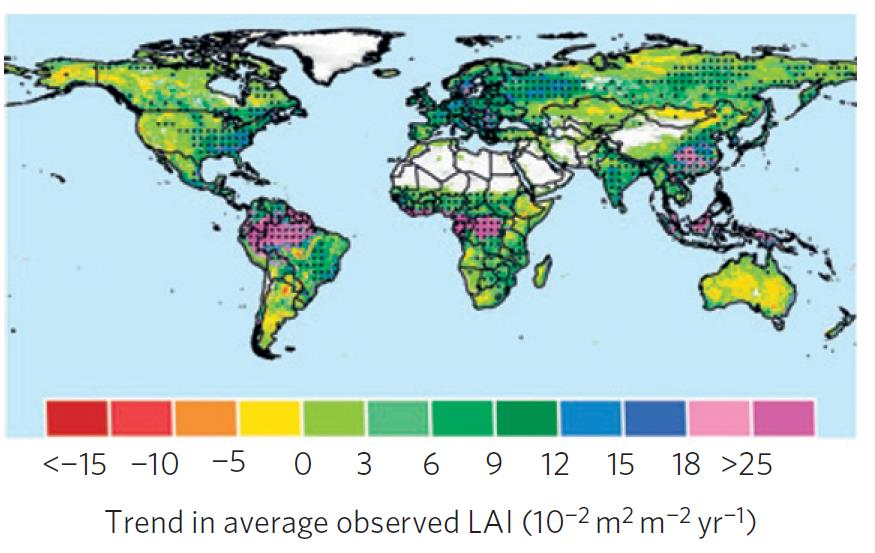
\includegraphics[width=1.0\textwidth]{bilder/bilderKlima-0002.jpg}\\[1cm]
\end{center}
\caption{Trends beim durchschnittlichen Blattflächenindex (LAI). Quelle: Zhu et al. 2016 Abbildung 3.}
\end{figure}

Piao et al. (2020) und Chen et al. (2024) berichten, dass der Ergrünungstrend ohne Anzeichen einer Verlangsamung fortsetzt, und CO$_2$-Düngung bleibt der dominante Treiber.

\subsection{Photosynthese und CO$_2$-Konzentrationen}

Pflanzen bauen Biomasse durch Photosynthese auf, einen Prozess, der Kohlendioxid, Wasser und Licht in Zucker umwandelt. Das für die Photosynthese verantwortliche Pflanzenenzym ist Ribulose-1,5-bisphosphat-carboxylase/oxygenase oder \emph{Rubisco}. Photosynthese wird eingeleitet, wenn CO$_2$ an der Oberfläche des Rubisco-Enzyms verfügbar ist, wo es in ein Molekül mit 3 Kohlenstoffatomen umgewandelt und danach in die Pflanzenmasse eingebaut wird. Dies wird als \emph{C3}-Prozess bezeichnet.

Rubisco wird geschätzt, vor etwa 3 Milliarden Jahren entstanden zu sein. Über geologische Zeit waren die atmosphärischen CO$_2$-Konzentrationen der Erde normalerweise viele Male höher als heute. Vor etwa 400 Millionen Jahren lagen CO$_2$-Konzentrationen schätzungsweise bei 2.000-4.000 ppm und waren für den größten Teil des Zeitraums von 200 bis 50 Millionen Jahren bei oder über 1.000 ppm (Berner 2006, Judd et al. 2024). Über die letzten 35 Millionen Jahre ist die atmosphärische CO$_2$-Konzentration stetig gefallen und fiel auf bis zu 170 ppm während Vereisung (Gerhart und Ward 2010). Während die moderne Änderungsrate von CO$_2$ im Vergleich zu früheren Zeiträumen hoch sein mag, zeigen die geologischen Beweise, dass Pflanzen und Tiere sich unter viel höheren CO$_2$-Konzentrationen als gegenwärtig entwickelten.

Als Antwort auf niedrige CO$_2$-Bedingungen entwickelten einige Pflanzen einen anderen photosynthetischen Weg namens \emph{C4}, bei dem CO$_2$ in der Nähe von Rubisco konzentriert wird, wodurch der \emph{C3}-Prozess effizienter funktionieren kann. Für landwirtschaftliche Zwecke sind die Pflanzenkategorien:
\begin{itemize}
\item C3: Reis, Weizen, Sojabohnen und die meisten anderen Feldfrüchte
\item C4: Mais, Zuckerrohr, Hirse, Sorghum	
\end{itemize}

Hätten atmosphärische CO$_2$-Konzentrationen weiter abgenommen, wäre das Pflanzenwachstum zurückgegangen und schließlich aufgehört. Unter \SI{180}{ppm} sind die Wachstumsraten vieler C3-Arten um 40-60 Prozent im Vergleich zu \SI{350}{ppm} reduziert (Gerhart und Ward 2010), und das Wachstum ist unter experimentellen Bedingungen von \SIrange{60}{140}{ppm} CO$_2$ vollständig zum Stillstand gekommen. Einige C4-Pflanzen können noch bei Konzentrationen von nur \SI{10}{ppm} wachsen, wenn auch sehr langsam (Gerhart und Ward 2010).


\begin{figure}[H]
\begin{center}
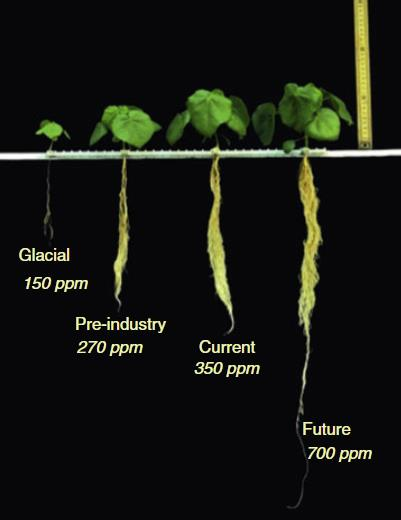
\includegraphics[width=0.6\textwidth]{bilder/bilderKlima-0003.jpg}\\[1cm]
\end{center}
\caption{Wachstum von \emph{Abutilon theophrasti} nach 14 Tagen unter identischen Bedingungen, jedoch mit den
angegebenen Schwankungen des CO2-Gehalts. Quelle: Gerhart und Ward (2010). Hinweis: „Aktuell” entspricht
1988 im Bild.}
\end{figure}

Die aktuellen CO$_2$-Konzentrationen liegen bei etwa \SI{430}{ppm}, gegenüber \SI{280}{ppm} in den frühen 1800er Jahren. Die positive Reaktion von Pflanzen auf zusätzliches CO$_2$ ist in Abbildung 2.2 dargestellt, reproduziert aus Gerhart und Ward (2010). Sie zeigt den Wachstumseffekt von CO$_2$ auf Samtpappel (Abutilon theophrasti) Sämlinge über 14 Tage unter kontrollierten Bedingungen, wo nur die CO$_2$-Exposition variiert wird. Die Zuwächse durch Erhöhung von CO$_2$ von \SI{150}{ppm} auf \SI{350}{ppm} setzen sich bei einer weiteren Verdopplung auf \SI{700}{ppm} fort.

Über die letzten 60+ Jahre gab es Tausende von Studien über die Reaktion von Pflanzen auf steigende CO$_2$-Konzentrationen. Das überwältigende Thema ist, dass Pflanzen, besonders C3-Pflanzen, von zusätzlichem CO$_2$ profitieren. Es gibt zwei Mechanismen, durch die CO$_2$ einen Wachstumsvorteil verleiht:

\begin{itemize}
\item Verstärkte Photosynthese über die oben beschriebenen Stoffwechselwege.
\item Erhöhte Wassernutzungseffizienz. Dies entsteht, weil Pflanzen CO$_2$ aufnehmen, indem sie die Stomata (Poren) auf der Blattoberfläche öffnen. Wenn CO$_2$ knapp ist, müssen die Stomata für lange Zeiträume weit offen gehalten werden, wodurch Wasser verdunsten kann. Unter angereicherten CO$_2$-Bedingungen bleiben die Stomata für längere Zeiträume geschlossen, wodurch die Pflanze Wasser länger zurückhalten kann und so die Wassernutzungseffizienz erhöht wird.
\end{itemize}

Spezifische Auswirkungen des Klimawandels auf die US-Landwirtschaft werden in Kapitel 9 überprüft.

\subsection{Steigendes CO$_2$ und Wassernutzungseffizienz von Feldfrüchten}

Deryng et al. (2016) untersuchten Beweise zur Wasserproduktivität von Feldfrüchten (CWP), dem Ertrag pro verwendete Wassereinheit, und lenkten Aufmerksamkeit auf das Potenzial von CO$_2$, sowohl die Photosynthese zu verstärken als auch die Transpiration auf Blattebene (Wasserverlust während der Blattatmung) zu reduzieren. Sie untersuchten alle verfügbaren FACE-Daten (Free Air CO$_2$ Enrichment—siehe Kapitel 9) zu Feldfruchtertragsänderungen für Mais, Weizen, Reis und Sojabohnen und kombinierten sie mit Feldfruchtemodell-Daten, die Ertragsreaktionen bis 2080 unter dem extremen RCP8.5-Emissionsszenario in vier Anbauregionen (Tropen, Trocken, Gemäßigt und Kalt) simulierten, von denen jede in regenabhängige und bewässerte Unterregionen aufgeteilt war. Sie berichteten, dass Modelle ohne CO$_2$-Düngung CWP-Verluste in jeder Region vorhersagten, aber diese wurden durch CO$_2$-Düngung mehr als ausgeglichen, sodass alle Regionen einen Netto-CWP-Gewinn zeigten.

Deryng et al. (2016) berichteten auch, dass negative Auswirkungen der Erwärmung auf Weizen- und Sojabohnenerträge vollständig durch CWP-Gewinne ausgeglichen und um bis zu 90 Prozent für Reis und 60 Prozent für Mais gemildert wurden.

Ähnlich bemerkten Cheng et al. (2017), dass die erhöhte Bruttoprimärproduktion von 1982 bis 2011 aufgrund steigender CO$_2$-Aufnahme von so großen CWP-Gewinnen begleitet war, dass der globale Wasserverbrauch von Pflanzen nicht gestiegen war, trotz der zusätzlichen Biomasse.

Deryng et al. (2016) nahmen an, dass Klimawandel \emph{Wasserknappheit verschärfen} würde. Doch während Modelle vorhersagen, dass Trockengebiete sich unter Klimaerwärmung ausdehnen werden, zeigen aktuelle Daten das Gegenteil: Ergrünung geschieht sogar in trockenen Gebieten. Zhang et al. (2024) berichten, dass aufgrund erhöhter CO$_2$-Konzentrationen \emph{zunehmende Trockenheit in Trockengebieten nicht zu einem allgemeinen Verlust der Vegetationsproduktivität führen wird}; höchstens 4 Prozent der derzeit trockenen Gebiete werden erhöhte Wüstenbildung erleben.

\subsection{CO$_2$-Düngungsvorteile in IPCC-Berichten}

Das IPCC hat globale Ergrünung und CO$_2$-Düngung landwirtschaftlicher Feldfrüchte nur minimal diskutiert. Das Thema wird kurz an einigen Stellen im Hauptteil des 6. und früherer IPCC-Bewertungsberichte anerkannt, aber in allen Zusammenfassungsdokumenten weggelassen. Abschnitt 2.3.4.3.3 des AR6 Working Group I-Berichts, betitelt \emph{globale Ergrünung und Bräunung}, weist darauf hin, dass der IPCC-Sonderbericht über Klimawandel und Land mit hoher Zuversicht geschlossen hatte, dass Ergrünung global über die letzten 2-3 Jahrzehnte zugenommen hatte. Er diskutiert dann, dass es Variationen im Ergrünungstrend zwischen Datensätzen gibt, und schließt, dass sie zwar hohe Zuversicht haben, dass Ergrünung aufgetreten ist, aber niedrige Zuversicht in das Ausmaß des Trends. Es gibt auch kurze Erwähnungen von CO$_2$-Düngungseffekten und Verbesserungen der Wassernutzungseffizienz in einigen anderen Kapiteln der AR6 Working Groups I und II-Berichte.

Insgesamt diskutieren jedoch die Policymaker Summaries, Technical Summaries und Synthesis Reports von AR5 und AR6 das Thema nicht.


\section{Die alkalischen Ozeane}

\subsection{Verändernder pH-Wert}

Eine neutrale wässrige Lösung hat einen pH-Wert von 7,0, während eine mit pH größer als 7,0 alkalisch (auch basisch genannt) und mit pH kleiner als 7,0 sauer ist. Der heutige globale Durchschnitts-pH-Wert von Oberflächenmeerwasser wird auf 8,04 geschätzt (\emph{Copernicus Marine Service 2025}, Abbildung 2.3), gegenüber einem geschätzten Wert von 8,2 in vorindustrieller Zeit (Gattuso und Hansson, 2011). Als CO$_2$-Konzentrationen in der Atmosphäre stiegen, absorbierten die Ozeane mehr, was ihren pH-Wert senkt. Abhängig von der Pufferkapazität der Ozeane wird erwartet, dass sie mit der Zeit etwas weniger alkalisch werden, was mit dem beobachteten pH-Rückgang übereinstimmt.

\begin{figure}[H]
\begin{center}
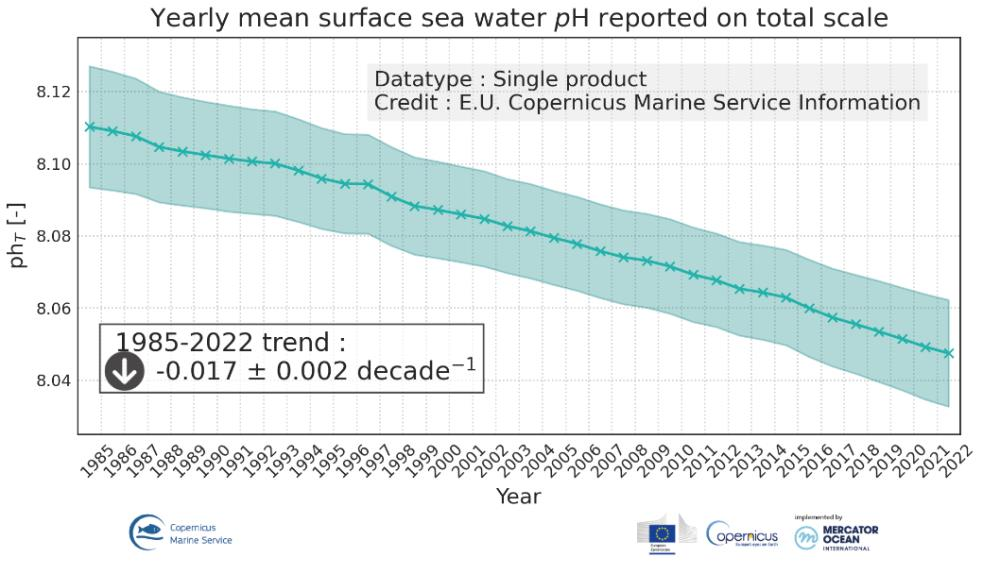
\includegraphics[width=0.8\textwidth]{bilder/bilderKlima-0004.jpg}\\[1cm]
\end{center}
\caption{pH-Wert der Ozeane 1985–2022. Quelle: Copernicus Marine Service 2025}
\end{figure}

Während dieser Prozess oft \emph{Ozeanversauerung} genannt wird, ist das eine Fehlbezeichnung, weil nicht erwartet wird, dass die Ozeane sauer werden; \emph{Ozeanneutralisierung} wäre genauer. Selbst wenn das Wasser sauer würde, wird angenommen, dass sich Leben in den Ozeanen entwickelte, als die Ozeane leicht sauer mit pH 6,5 bis 7,0 waren (Krissansen-Totton et al., 2018). Auf der Zeitskala von Tausenden von Jahren zeigen Bor-Isotop-Proxy-Messungen, dass der Ozean-pH-Wert während der letzten Vereisung (bis vor etwa 20.000 Jahren) um 7,4 oder 7,5 lag und auf heutige Werte anstieg, als sich die Welt während der Enteisung erwärmte (Rae et al., 2018). Somit scheinen Ozeanbiota widerstandsfähig gegenüber natürlichen langfristigen Veränderungen des Ozean-pH-Werts zu sein, da Meeresorganismen einer weiten Bandbreite von pH-Werten ausgesetzt waren.

\subsection{Korallenriff-Veränderungen}

Es gibt Bedenken, dass ein abnehmender pH-Wert des Meerwassers die Verkalkungsrate von Korallenriffen reduzieren wird. Aber Korallenriffe ertragen bereits große pH-Schwankungen, teilweise aufgrund täglicher photosynthetischer Aktivität im Riff; gemessene pH-Werte reichen von 9,4 während des Tages bis 7,5 nachts (Revelle und Fairbridge, 1957). De'ath et al. (2009) berichteten, dass Verkalkungsraten am Great Barrier Reef von 1990 bis 2005 um 14,2 Prozent zurückgegangen waren. Ridd et al. (2013) verwendeten jedoch andere Methoden und fanden keinen signifikanten Trend in den Verkalkungsraten.

Jüngste Daten vom Australian Institute of Marine Science zeigen, dass sich das Great Barrier Reef stark erholt hat. Der Korallenbedeckungsgrad erreichte 2022 36-Jahres-Höchststände in zwei Dritteln des Riffs. Das Institute kommentierte: \emph{Das war das dritte Jahr in Folge mit weit verbreiteter Erholung} (Australian Institute of Marine Science, 2022). Die \emph{Woods Hole Oceanographic Institution} bemerkte 2023: \emph{Das Great Barrier Reef macht ein bemerkenswertes Comeback} (Woods Hole Oceanographic Institution, 2023).

\begin{figure}[H]
\begin{center}
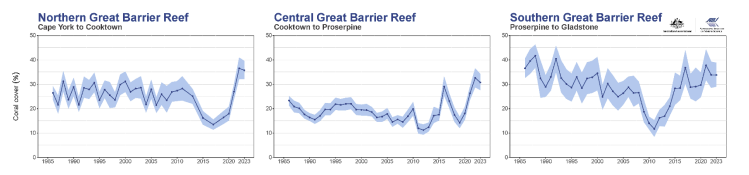
\includegraphics[width=1.0\textwidth]{bilder/bilderKlima-0005.png}\\[1cm]
\end{center}
\caption{Hartkorallenbedeckung in drei Regionen des \emph{Great Barrier Reef} von 1985 bis 2023. Quelle: AIMS 2023.}
\end{figure}

Es scheint, dass Korallen anpassungsfähiger sind als früher gedacht. Die Vorfahren moderner Korallen erschienen vor etwa 245 Millionen Jahren. CO$_2$-Konzentrationen waren für mehr als 200 Millionen Jahre danach viele Male höher als heute. Ein Großteil der öffentlichen Diskussion über die Auswirkungen der Ozean-"Versauerung" auf Meeresbiota war einseitig und übertrieben.

Ähnlich fand eine Meta-Analyse (Clements et al., 2021) der negativen Auswirkungen der Ozeanversauerung auf das Verhalten von Rifffischen das, was sie einen \emph{Decline-Effekt} nannten: anfänglich dramatische Schlussfolgerungen, die in prominenten Zeitschriften veröffentlicht wurden und scheinbar große Auswirkungen der Versauerung zeigten, tendierten dazu, von nachfolgenden Studien mit größeren Stichprobengrößen gefolgt zu werden, die viel kleinere und typischerweise nicht-existente Effekte ergaben. Sie fordern ihre Kollegen auf, Forschungspraktiken zu verbessern, um dem \emph{Decline-Effekt} entgegenzuwirken:

Die überwiegende Mehrheit der Studien mit großen Effektgrößen in diesem Bereich tendiert dazu, durch niedrige Stichprobengrößen charakterisiert zu sein, wird aber dennoch in hochrangigen Zeitschriften veröffentlicht und hat einen unverhältnismäßigen Einfluss auf das Feld in Bezug auf Zitationen. Wir behaupten, dass Ozeanversauerung einen vernachlässigbaren direkten Einfluss auf Fischverhalten hat, und wir setzen uns für verbesserte Ansätze ein, um das Potenzial für einen Decline-Effekt in zukünftigen Forschungsrichtungen zu minimieren (Clements et al., 2021).

Zusammenfassend ist Meeresleben komplex, und vieles davon entwickelte sich, als die Ozeane relativ zur Gegenwart sauer waren. Die Vorfahren moderner Korallen erschienen vor etwa 245 Millionen Jahren. CO$_2$-Konzentrationen waren für mehr als 200 Millionen Jahre danach viele Male höher als heute. Ein Großteil der öffentlichen Diskussion über die Auswirkungen der Ozean-"Versauerung" auf Meeresbiota war einseitig und übertrieben.

\vfill
{\textbf Literaturverzeichnis:}

AR6: Intergovernmental Panel on Climate Change Sixth Assessment Report (2021) Working Group I Contribution. www.ipcc.ch.

Australian Institute of Marine Science. (2022). Continued coral recovery leads to 36-year highs across two-thirds of the Great Barrier Reef. \url{https://www.aims.gov.au/sites/default/files/2022-08/AIMS_LTMP_Report_on\%20GBR_coral_status_2021_2022_040822F3.pdf}

Beeden, R., Maynard, J., Puotinen, M., Marshall, P., Dryden, J., Goldberg, J., and Williams, G. (2015). Impacts and recovery from Severe Tropical Cyclone Yasi on the Great Barrier Reef. PLOS ONE, 10, e0121272. https://doi.org/10.1371/journal.pone.0121272

Berner, R. A. (2006). GEOCARBSULF: A combined model for Phanerozoic atmospheric O$_2$ and CO$_2$. Geochimica et Cosmochimica Acta, 70, 5653–5664.

Browman, H. I. (2016). Applying organized scepticism to ocean acidification research. ICES Journal of Marine Science, 73(3), 529.1–536. https://doi.org/10.1093/icesjms/fsw010

Chen, C., Park, T., Wang, X., Piao, S., Xu, B., Chaturvedi, R. K., and Myneni, R. B. (2019). China and India lead in greening of the world through land-use management. Nature Sustainability, 2, 122–129. https://www.nature.com/articles/s41893-019-0220-7

Chen, X., Wang, Y., Liu, Y., and Piao, S. (2024). The global greening continues despite increased drought stress since 2000. Global Ecology and Conservation, 49, e02791. https://www.sciencedirect.com/science/article/pii/S2351989423004262

Cheng, L., Zhang, L., Wang, Y. P., et al. (2017). Recent increases in terrestrial carbon uptake at little cost to the water cycle. Nature Communications, 8, 110. https://doi.org/10.1038/s41467-017-00114-5

Clements, J. C., Sundin, J., Clark, T. D., and Jutfelt, F. (2022). Meta-analysis reveals an extreme "decline effect" in the impacts of ocean acidification on fish behavior. PLOS Biology, 20(2), e3001511. https://doi.org/10.1371/journal.pbio.3001511

Copernicus Marine Service. (2025). Global ocean acidification – Mean sea water pH time series and trend from multi-observations reprocessing. \url{https://data.marine.copernicus.eu/product/GLOBAL_OMI_HEALTH_carbon_ph_area_averaged/description}

De'ath, G., Lough, J., and Fabricius, K. (2009). Declining coral calcification on the Great Barrier Reef. Science, 323, 116–119. https://doi.org/10.1126/science.1165283

Deryng, D., Conway, D., Ramankutty, N., Price, J., Warren, R., Jones, R., ... and Elliott, J. (2016). Regional disparities in the beneficial effects of rising CO$_2$ concentrations on crop water productivity. Nature Climate Change. https://doi.org/10.1038/nclimate2995

Gattuso, J. P., and Hansson, L. (Eds.). (2011). Ocean acidification: Background and history. Oxford University Press.

Gerhart, L. M., and Ward, J. K. (2010). Plant responses to low [CO$_2$] of the past. New Phytologist, 188, 674–695. https://nph.onlinelibrary.wiley.com/doi/pdf/10.1111/j.1469-8137.2010.03441.x

Haverd, V., B. Smith, J. G. Canadell, et al. (2020). Higher than expected CO$_2$ fertilization inferred from leaf to global observations. Global Change Biology, 26, 2390–2402. https://doi.org/10.1111/gcb.14950

Keenan, T. F., X. Luo, B. D. Stocker, et al. (2023). A constraint on historic growth in global photosynthesis due to rising CO2. Nature Climate Change 13(12): 1376-1381 DOI: 10.1038/s41558-023-01867-2.

Judd, E. J., Scotese, C. R., Young, S. A., et al. (2024). A 485-million-year history of Earth's surface temperature. Science, 385(6715). https://doi.org/10.1126/science.adk3705

Krissansen-Totton, J., Arney, G. N., and Catling, D. C. (2018). Constraining the climate and ocean pH of the early Earth with a geological carbon cycle model. Proceedings of the National Academy of Sciences, 115(6), 4105–4110. https://doi.org/10.1073/pnas.1721296115

Piao, S., X. Wang, T. Park, et al. (2020). Characteristics, drivers and feedbacks of global greening. Nature Reviews Earth \& Environment 1(1): 14-27 DOI: 10.1038/s43017-019-0001-x

Rae, J. W. B., Burke, A., Robinson, L. F., et al. (2018). CO$_2$ storage and release in the deep Southern Ocean on millennial to centennial timescales. Nature, 562, 569–573. https://doi.org/10.1038/s41586-018-0614-0

Revelle, R., and Fairbridge, R. W. (1957). Carbonate and carbon dioxide. In J. W. Hedgpeth (Ed.), Treatise on marine ecology and paleoecology (Vol. 1). Geological Society of America.

Ridd, P., Silva, E., and Stieglitz, T. (2013). Have coral calcification rates slowed in the last twenty years? Marine Geology, 346, 392–399. https://doi.org/10.1016/j.margeo.2013.09.002

Woods Hole Oceanographic Institution. (2023). Is the Great Barrier Reef making a comeback? https://www.whoi.edu/oceanus/feature/is-the-great-barrier-reef-making-a-comeback/

Zeng, Z., Piao, S. Li, L., et al. (2017). Climate mitigation from vegetation biophysical feedbacks during the past three decades. Nature Climate Change. https://doi.org/10.1038/nclimate3299

Zhang, Y., Liu, Y., Chen, X., et al. (2024). Less than 4% of dryland areas are projected to desertify despite increased aridity under climate change. Nature Communications Earth and Environment, 5. https://www.nature.com/articles/s43247-024-01463-y

Zhu, Z., Piao, S., Myneni, R. B., et al. (2016). Greening of the Earth and its drivers. Nature Climate Change, 6, 791–795. https://www.nature.com/articles/nclimate3004

%\numberwithin{figure}{section}
\FigureNumbersBySection
\chapter{Menschliche Einflüsse auf das Klima}
\paragraph{Kapitelzusammenfassung}
\begin{quote}
Das globale Klima ist natürlicherweise auf allen Zeitskalen variabel. Anthropogene CO$_2$-Emissionen verstärken diese Variabilität, indem sie die gesamte Strahlungsenergiebilanz in der Atmosphäre verändern.

Das IPCC hat die Rolle der Sonne beim Klimawandel herabgespielt, aber es gibt plausible Rekonstruktionen der Sonneneinstrahlung, die darauf hindeuten, dass sie zur jüngsten Erwärmung beigetragen hat.

Klimaprojektionen basieren auf IPCC-Emissionsszenarien, die dazu tendierten, beobachtete Trends zu übertreffen. Die meisten akademischen Klimaauswirkungsstudien der letzten Jahre basieren auf dem extremen RCP 8.5-Szenario, das jetzt als unplausibel gilt; seine Verwendung als Business-as-usual-Szenario war irreführend.

Kohlenstoffkreislaufmodelle verbinden jährliche Emissionen mit dem Wachstum des atmosphärischen CO$_2$-Bestands. Während sich Modelle über die Rate der Land- und Ozean-CO$_2$-Aufnahme uneinig sind, stimmen alle darin überein, dass sie seit 1959 gestiegen ist.

Es gibt Belege dafür, dass Urbanisierungsverzerrungen in der Landerwärmungsaufzeichnung nicht vollständig aus Klimadatensätzen entfernt wurden.
\end{quote}

\section{Komponenten der Strahlungsantriebe und ihre Geschichte}
\subsection{Historischer Strahlungsantrieb}
Ein sich veränderndes Klima war die Norm während der gesamten 4.6 Milliarden Jahre langen Geschichte der Erde. Die Temperatur und Wettermuster der Erde verändern sich natürlich über Zeitskalen von Jahrzehnten bis zu Millionen von Jahren. Natürliche Variationen des Oberflächenklimas entstehen auf zwei Wegen. Interne Klimaschwankungen im Zusammenhang mit Zirkulationen in der Atmosphäre und den Ozeanen tauschen Energie, Wasser und Kohlenstoff zwischen der Atmosphäre, Ozeanen, Land und Eis aus. Externe Einflüsse auf das Klimasystem umfassen Variationen in der von der Sonne empfangenen Energie und die Auswirkungen von Vulkanausbrüchen. Menschliche Aktivitäten beeinflussen das Klima durch Veränderungen der Landnutzung und Landbedeckung. Menschen verändern auch die Zusammensetzung der Atmosphäre durch Emissionen von CO$_2$ und anderen Treibhausgasen und durch die Veränderung der Konzentration von Aerosolpartikeln in der Atmosphäre.

Die Erde wird durch das Sonnenlicht erwärmt, das sie absorbiert, und wird durch die Wärme gekühlt, die sie in den Weltraum abstrahlt. Über die Erdoberfläche gemittelt, beinhalten diese Prozesse jeweils Energieflüsse von etwa 240 Watt pro Quadratmeter (W/m²). Wenn sie im Gleichgewicht sind, gibt es keine äußeren Ursachen für Erwärmung oder Abkühlung. Sowohl menschliche als auch natürliche Einflüsse auf das Klima verändern dieses Gleichgewicht und verursachen damit Klimaveränderungen.

Einflüsse auf die Energiebilanz der Erde an der Spitze der Atmosphäre werden durch \emph{Strahlungsantrieb} quantifiziert, das Ausmaß, in dem sie das Erwärmungs-/Abkühlungsgleichgewicht stören; ein positiver Antrieb erwärmt, während ein negativer Antrieb kühlt. Die geschätzte Geschichte der wichtigsten Komponenten des Strahlungsantriebs seit 1750 durch das IPCC ist in den folgenden zwei Abbildungen aus seinem AR6 dargestellt.

\begin{figure}[H]
\begin{center}
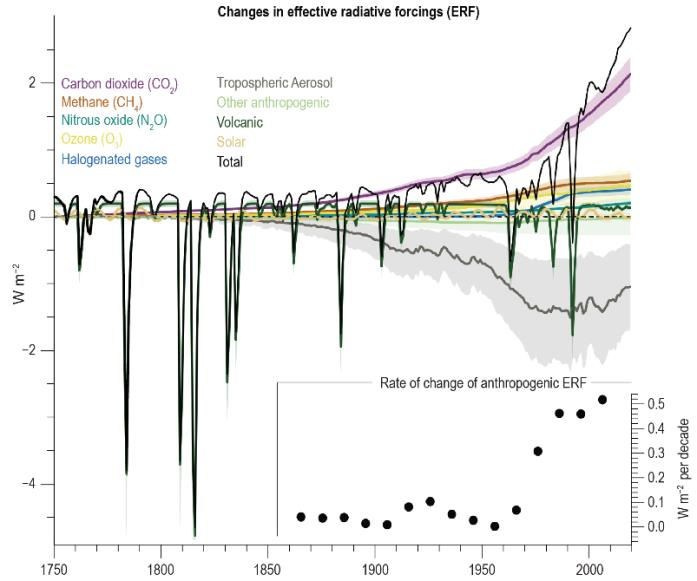
\includegraphics[width=1.0\textwidth]{bilder/bilderKlima-0006.jpg}\\[1cm]
\end{center}
\caption{IPCC-Schätzungen der Komponenten des Strahlungsantriebs im Zeitverlauf. Die Schattierung zeigt
die Unsicherheitsbereiche an. Quelle: AR6 WGI Ch2 Abb. 10}
\end{figure}

\begin{figure}[H]
\begin{center}
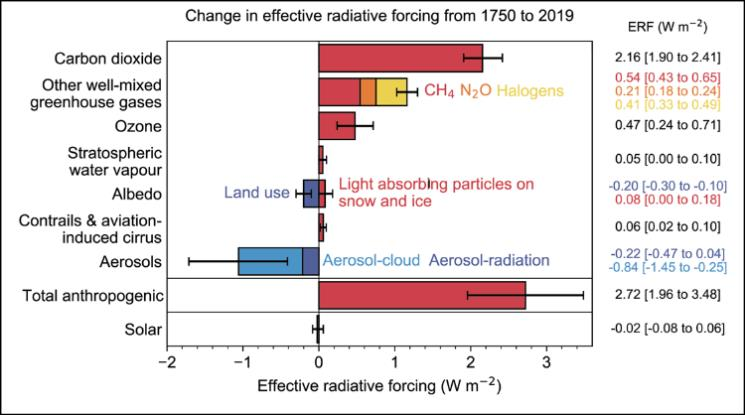
\includegraphics[width=1.0\textwidth]{bilder/bilderKlima-0007.jpg}\\[1cm]
\end{center}
\caption{IPCC-Schätzungen der Veränderungen der Strahlungsantriebskomponenten von 1750 bis 2019. Quelle:
AR6 WGI Kap. 7 Abb. 7-6.}
\end{figure}

Diese Grafiken zeigen, dass der gesamte Strahlungsantrieb sowohl aus natürlichen als auch aus anthropogenen Komponenten besteht. Kohlendioxid ist der größte menschliche Einfluss auf das Klima und derjenige, der am relevantesten für den Einfluss der Nutzung fossiler Brennstoffe ist. Es übt einen erwärmenden Einfluss aus, indem es die Kühlkraft der Atmosphäre verringert. CO$_2$-Emissionen akkumulieren in der Atmosphäre, wie im folgenden Abschnitt beschrieben, sodass der erwärmende Einfluss wächst.

Andere anthropogene Strahlungsantriebe umfassen andere Treibhausgase (Methan, Lachgas, fluorierte Gase), Aerosole und Landnutzungsänderungen. Es gibt jedoch erhebliche Unsicherheiten in diesen Komponenten. Das IPCC identifiziert Wolken-Aerosol-Wechselwirkungen als die größte Unsicherheit im gesamten Strahlungsantrieb.

Eine wichtige natürliche Komponente ist die Sonneneinstrahlung. Variationen in der Sonnenaktivität sind gut dokumentiert und können das Klima beeinflussen. Das IPCC hat jedoch die Rolle solarer Variabilität beim Klimawandel heruntergespielt. Soon et al. (2021) stellten fest, dass die Konsensaussagen des IPCC zum solaren Antrieb vorzeitig durch die Unterdrückung abweichender wissenschaftlicher Meinungen formuliert wurden.

Eine weitere natürliche Strahlungsantriebskomponente sind vulkanische Aerosole, die einen episodischen kühlenden Einfluss ausüben. Box 4.1 im IPCC AR6-Bericht behandelt die Klimaauswirkungen von Vulkanausbrüchen und bemerkt drei explosive Vulkanausbrüche, die in der ersten Hälfte des 19. Jahrhunderts auftraten. Dazu gehörte der Tambora-Ausbruch von 1815, der zum 'Jahr ohne Sommer' führte, mit mehreren Ernteausfällen in der gesamten Nordhalbkugel. Es gibt Unsicherheit über das Vorzeichen der relativ kleinen Antriebskraft des Unterwasservulkans Hunga Tonga, der 2022 ausbrach (Jenkins et al. 2023, Schoeberl et al. 2024).

Abbildung 3.1.1 zeigt, dass die anthropogene Antriebskomponente vor etwa 1900 vernachlässigbar war und seitdem stetig gestiegen ist und heute auf fast \SI{3}{\watt\per\square\meter} angestiegen ist. Dies ist jedoch immer noch nur etwa 1 Prozent der ungestörten Strahlungsflüsse, was es zu einer Herausforderung macht, die Auswirkungen des anthropogenen Antriebs zu isolieren; modernste Satellitenschätzungen globaler Strahlungsenergieflusse sind nur auf wenige \si{\watt\per\square\meter} genau.

Natürliche Quellen globaler Energieungleichgewichte außer Vulkanen und der gesamten Sonneneinstrahlung (TSI) sind in diesen Grafiken nicht enthalten, da sie weitgehend unbekannt bleiben.

\subsection{Veränderung des atmosphärischen CO$_2$ seit 1958}

Der erwärmende Einfluss von Kohlendioxid hängt davon ab, wie viel \emph{zusätzliches} CO$_2$ sich in der Atmosphäre ansammelt – d.h. seine Konzentration über dem vorindustriellen Wert von \SI{280}{ppm}. Der CO$_2$-Gehalt, wie er am Mauna Loa-Observatorium in Hawaii aufgezeichnet wird, der allgemein als repräsentative globale Durchschnittskonzentration verwendet wird, ist online verfügbar unter \url{https://gml.noaa.gov/ccgg/trends/index.html}. Die Konzentration lag zu Beginn der Aufzeichnung 1959 bei etwa \SI{316}{ppm} und liegt jetzt bei etwa \SI{430}{ppm}, ein Anstieg von 36 Prozent. Am Ende der letzten Vereisung waren die CO$_2$-Konzentrationen auf etwa \SI{180}{ppm} gefallen. Wie in Kapitel 2 diskutiert, beginnen C3-Pflanzen bei CO$_2$-Konzentrationen unter etwa \SI{140}{ppm} zu sterben und C4-Pflanzen bei Konzentrationen unter \SI{100}{ppm}, sodass bei weiterem Fallen der CO$_2$-Konzentrationen das Pflanzenleben gefährdet gewesen wäre.


\begin{figure}[H]
\begin{center}
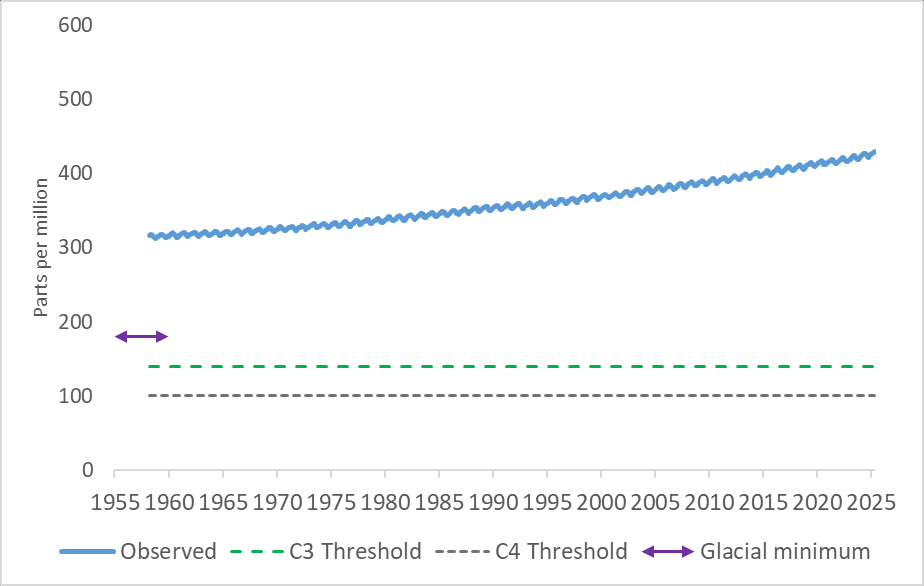
\includegraphics[width=1.0\textwidth]{bilder/bilderKlima-0009.png}\\[1cm]
\end{center}
\caption{Jährliche durchschnittliche CO2-Konzentrationen in der Atmosphäre (1959–2025) in ppm, gemessen am
Mauna Loa (blau). C3-Schwellenwert: Wert, unterhalb dessen C3-Pflanzen zu sterben beginnen (140 ppm, siehe
Kapitel 2). C4-Schwellenwert: Wert, unterhalb dessen C4-Pflanzen zu sterben beginnen (100 ppm, siehe Kapitel 2).
Glaziales Minimum: Mindestniveau während der letzten Eiszeiten (lila Pfeil). CO2-Datenquelle:
\url{https://gml.noaa.gov/ccgg/trends/index.html}}
\end{figure}

Der jährliche Konzentrationsanstieg ist nur etwa die Hälfte des emittierten CO$_2$, weil Land- und Ozeanprozesse derzeit \emph{überschüssiges} CO$_2$ mit einer Rate von etwa 50 Prozent der menschlichen Emissionen absorbieren. Zukünftige Konzentrationen und damit zukünftige menschliche Einflüsse auf das Klima hängen daher von zwei Komponenten ab: (1) zukünftige Raten globaler menschlicher CO$_2$-Emissionen und (2) wie schnell Land und Ozean zusätzliches CO$_2$ aus der Atmosphäre entfernen. Wir diskutieren jede dieser der Reihe nach.

\section{Zukünftige Emissionsszenarien und der Kohlenstoffkreislauf}

\subsection{Emissionsszenarien}

Die Bewertung der Gefahren zukünftiger THG-Emissionen erfordert Annahmen darüber, was diese Emissionen sein werden. Zukünftige Emissionen und damit menschliche Einflüsse auf das Klima werden von zukünftiger Demografie, Wirtschaftstätigkeit, Regulierung sowie Energie- und Agrartechnologien abhängen. Verschiedene Annahmen über jeden dieser Faktoren führen zu Projektionen von Treibhausgasemissionen und -konzentrationen, Aerosolkonzentrationen und Veränderungen der Landnutzung, die letztendlich zu Annahmen über anthropogenen Strahlungsantrieb kombiniert werden können.

Die großen Unsicherheiten über diese vielen Faktoren machen es unmöglich, zukünftige Emissionen präzise vorherzusagen. Stattdessen hat das IPCC verschiedene Szenario-Sets verwendet, die einen plausiblen Bereich von Möglichkeiten für Bevölkerung, Wirtschaft und Technologien abdecken sollen. Jüngste Versionen der Szenarien sind durch eine Zahl gekennzeichnet, die den anthropogenen Strahlungsantrieb angibt, der 2100 unter diesem Szenario erwartet wird. So entspricht ein mit "6" bezeichnetes Szenario \SI{6}{\watt\per\square\meter} menschlich induziertem Strahlungsantrieb (Erwärmung) am Ende des Jahrhunderts. (Erinnern Sie sich, der aktuelle anthropogene Strahlungsantrieb beträgt etwa \SI{2.7}{\watt\per\square\meter}.)

Obwohl das IPCC nicht behauptet, dass seine Emissionsszenarien Vorhersagen sind, werden sie oft als solche behandelt. Vergleiche vergangener Szenario-Gruppen mit Beobachtungen zeigen, dass IPCC-Emissionsprojektionen dazu tendierten, tatsächliche nachfolgende Emissionen zu überschätzen. Für den dritten und vierten IPCC-Bewertungsbericht wurde eine Reihe von Emissionsprojektionen aus dem Sonderbericht zu Emissionsszenarien verwendet; diese wurden als SRES-Szenarien bezeichnet. McKitrick et al. (2012) zeigten, dass die SRES-Szenario-Emissionsverteilung bei Umrechnung in Pro-Kopf-Werte im Vergleich zu beobachteten Trends nach oben verzerrt war. Die Verzerrung der SRES-Szenarien wurde durch die spätere Analyse von Hausfather et al. (2019) bestätigt, die zeigten, dass beobachtete atmosphärische CO$_2$-Konzentrationen dem unteren Ende des SRES-Bereichs und auch nachfolgender IPCC-Szenario-Bereiche folgten (Abbildung 3.2.1).

Für AR5 entwickelte das IPCC ein neues Set von Szenarien, die \emph{Representative Concentration Pathways} (RCPs) genannt wurden. Diese wurden durch eine Zahl identifiziert, die den Anstieg im Antrieb repräsentierte, und wurden daher RCP2.6, RCP4.5, RCP6.0 und RCP8.5 genannt. RCP2.6 (was einen anthropogenen Strahlungsantrieb 2100 von \SI{2.6}{\watt\per\square\meter} impliziert) beschreibt einen THG-Konzentrationspfad, der zu einer Erwärmung deutlich unter 2°C führt. Am anderen Ende der Skala ist RCP8.5 ein extremes Ergebnis, das fast \SI{5}{\celsius} Erwärmung von 1900 bis 2100 impliziert.

RCP8.5 kam dazu, als \emph{No-Policy-Baseline} oder \emph{Business-as-usual}-Szenario sowohl in der akademischen Literatur als auch in den populären Medien bezeichnet zu werden. Es wurde daher verwendet, um das Referenzergebnis zu generieren, das angeblich die Welt des 21. Jahrhunderts in Abwesenheit zunehmend strenger Emissionsreduktionspolitiken repräsentiert. Aber RCP8.5 war als ein Niedrig-Wahrscheinlichkeits-Hochemmissionsszenario gedacht, und seine Verwendung als Business-as-usual-Baseline wurde als grob irreführend kritisiert.\footnote{Dieses extreme Szenario ist nützlich für Modellierer, da ein großer Antrieb eine große Antwort (Erwärmung) generiert, was es einfacher macht, die Sensitivität eines Modells zu bewerten. Aber das ist sehr unterschiedlich davon, zu behaupten, es sei ein plausibles zukünftiges Ergebnis.} Hausfather und Peters (2020a), die in einem Kommentar in Nature schrieben, wiesen darauf hin, dass RCP8.5 als ein extremer Worst-Case entwickelt wurde, und sein Missbrauch als \emph{Business as usual}-Baseline hat zu einer großen Anzahl irreführender Studien und Medienberichterstattung geführt.

Die Unplausibilität des RCP8.5-Szenarios wurde von Burgess et al. (2021) untersucht. Die Unplausibilität von RCP8.5 sollte nicht als sehr unwahrscheinlich (z.B. 95. Perzentil) oder ein \emph{Worst Case} interpretiert werden, sondern eher als genuinen unplausibel aufgrund der Unplausibilität der Inputs, die erforderlich sind, um einen Antrieb von \SI{8.5}{\watt\per\square\meter} zu erreichen. Sie bemerkten, dass RCP8.5 bereits von beobachteten Trends in der Energienutzung abgewichen ist und die nahen zukünftigen Trends scharf von denen der Internationalen Energieagentur (IEA) abweichen, die marktbasierte Projektionen der Energienutzung für die kommenden Jahrzehnte bereitstellt. Pielke Jr. et al. (2022) zeigten weiter, dass die historischen und projizierten IEA-Trends nahe dem Boden der Umhüllungen sowohl der RCP-Projektionen als auch der jüngeren Shared Socioeconomic Pathway (SSP)-Szenario-Trends verlaufen.

Schwalm et al. (2020) verteidigten die Verwendung von RCP8.5 mit der Begründung, dass kumulative CO$_2$-Emissionen über 2005-2020 es enger verfolgen als die niedrigeren RCP-Szenarien. Sie argumentieren auch, dass eine modifizierte Version der IEA-Szenarien RCP8.5 in den kommenden Jahrzehnten eng verfolgt. Hausfather und Peters (2020b) antworteten, dass die Fertigkeit von RCP8.5 über diese 15 Jahre auf ausgleichende Fehler in seiner Repräsentation von CO$_2$ aus Brennstoffnutzung und Landnutzungsänderung zurückzuführen ist, und die scheinbare Übereinstimmung mit IEA in kommenden Jahrzehnten ist darauf zurückzuführen, dass Schwalm et al. sehr hohe Landnutzungsemissionen hinzufügten. Die eigenen projizierten CO$_2$-Emissionen der IEA verfolgen deutlich unter RCP8.5.

Weitverbreitete Verwendung von RCP8.5 als No-Policy-Baseline hat eine Verzerrung in Richtung Alarm in der Klimaauswirkungsliteratur geschaffen. Das Ausmaß dieses Problems wurde in einer Literaturanalyse von Pielke Jr. und Ritchie (2020) bestätigt. Sie fanden, dass etwa 16.800 wissenschaftliche Arbeiten, die zwischen 2010 und 2020 veröffentlicht wurden, das RCP8.5-Szenario verwendeten, wobei etwa 4.500 der Artikel RCP8.5 mit dem Konzept von \emph{Business-as-usual} verknüpften. Ihre Analyse zeigte, wie RCP8.5 nicht nur von einzelnen Forschern missbraucht wurde, sondern auch von einflussreichen Wissenschaftsagenturen wie dem IPCC und dem U.S. National Climate Assessment (USNCA), was direkt zu irreführender Berichterstattung in prominenten Medien geführt hat.

\begin{figure}[H]
\begin{center}
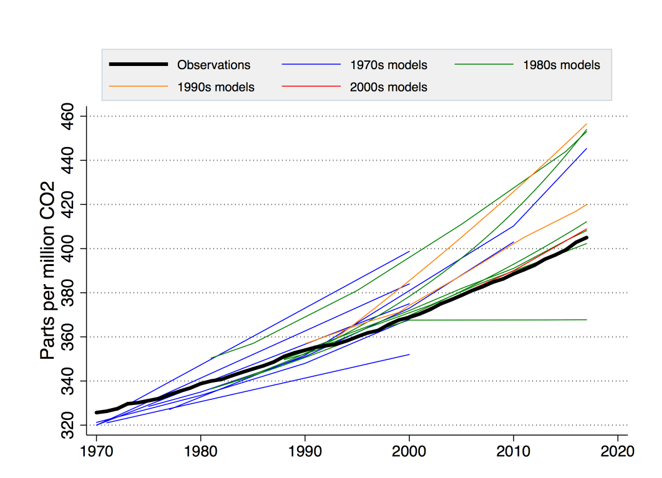
\includegraphics[width=1.0\textwidth]{bilder/bilderKlima-0011.png}\\[1cm]
\end{center}
\caption{Seit den 1970er Jahren haben aufeinanderfolgende Familien von Emissions- und Konzentrationsprognosen (farbige
Linien) die Beobachtungen (schwarze Linie) durchweg überschätzt. Quelle: Hausfather et al. (2019)
Abbildung S4.}
\end{figure}

Pielke und Ritchie (2020) berichteten, dass neue Studien, die RCP8.5 verwendeten, mit einer Rate von etwa 20 pro Tag veröffentlicht wurden, wobei etwa zwei pro Tag spezifisch RCP8.5 und \emph{business as usual} verknüpften. Sie schließen, dass die Klimaforschungsgemeinschaft ein Jahrzehnt damit verbracht hat, \emph{wissenschaftliche Ressourcen für Science Fiction zu verwenden} und dass \emph{Die wissenschaftliche Literatur ist in eine apokalyptische Richtung unausgewogen geworden.}

Das IPCC entwickelte ein neues Set von Szenarien für AR6, die \emph{Shared Socioeconomic Pathway} (SSP)-Szenarien, die die in den RCP- und SRES-Szenarien gezeigte Verzerrung fortgesetzt haben. Abbildung 3.2.2 zeigt die von der Internationalen Energieagentur (IEA) zusammengestellten gesamten globalen beobachteten CO$_2$-Emissionen, zusammengeführt mit der Emissionsprojektion der EIA unter Berücksichtigung von Energienutzungsprojektionen und aktuellen Politiken. Die anderen Linien zeigen den Bereich der IPCC SSP-Szenarien (SSP1-SSP5). Ab 2023 lagen globale CO$_2$-Emissionen deutlich unter SSP7.0 und waren sogar unter SSP2-4.5.

\begin{figure}[H]
\begin{center}
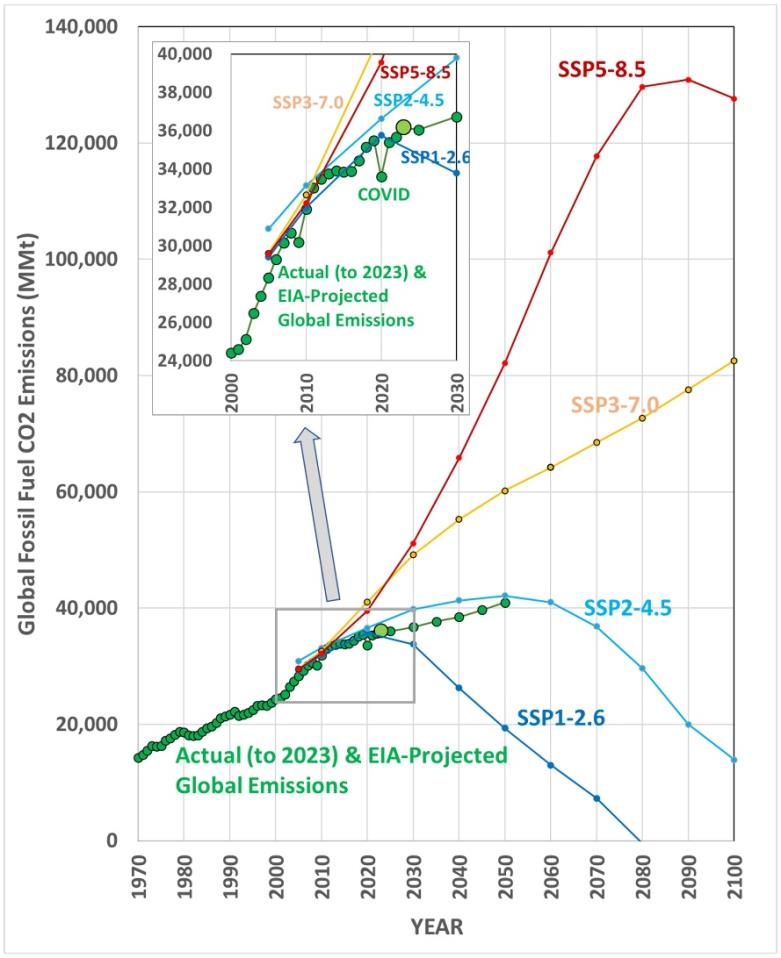
\includegraphics[width=1.0\textwidth]{bilder/bilderKlima-0012.jpg}\\[1cm]
\end{center}
\caption{Beobachtete und prognostizierte CO$_2$-Emissionen. Quelle: IPCC (SSP-Szenarien) und
Energy Information Administration (EIA). Grün: beobachtete historische Emissionen und EIA-Prognosen.
Andere Linien: SSP1-5. Datenquelle: Friedlingstein et al. (2024).}
\end{figure}

\subsection{Der Kohlenstoffkreislauf, der Emissionen und Konzentrationen in Beziehung setzt}
Kohlendioxidemissionen aus der Verbrennung fossiler Brennstoffe (und in geringerem Maße Entwaldung und Zementproduktion) haben zu stetig steigenden CO$_2$-Konzentrationen in der Atmosphäre geführt, wie in Abb. 3.1.3 gezeigt. Die Beziehung zwischen Emissionen und Konzentration wird durch den globalen Kohlenstoffkreislauf von Land- und Ozeanprozessen bestimmt, die Kohlenstoff mit der Atmosphäre austauschen. Unser Verständnis dieser Prozesse wurde von Crisp et al. (2021) überprüft.

Es gibt etwa \SI{850}{\giga\tonne} Kohlenstoff (\si{\giga\tonne\of{C}}) in der Erdatmosphäre\footnote{Weil CO$_2$ chemisch durch den Verlauf des Kohlenstoffkreislaufs transformiert wird, ist es zweckmäßiger, Kohlenstoffatome zu verfolgen statt CO$_2$-Moleküle. Eine Gigatonne Kohlenstoff (\si{\giga\tonne\of{C}}) entspricht etwa \SI{3.7}{\giga\tonne} CO$_2$.}, fast alles davon in der Form von CO$_2$. Jedes Jahr tauschen biologische Prozesse (Pflanzenwachstum und -zerfall) und physische Prozesse (Ozeanabsorption und -ausgasung) etwa \SI{200}{\giga\tonne\of{C}} dieses Kohlenstoffs mit der Erdoberfläche aus (ungefähr \SI{80}{\giga\tonne\of{C}} mit dem Land und \SI{120}{\giga\tonne\of{C}} mit den Ozeanen). Bevor menschliche Aktivitäten bedeutsam wurden, waren Entfernungen aus der Atmosphäre grob im Gleichgewicht mit Hinzufügungen. Aber die Verbrennung fossiler Brennstoffe (Kohle, Öl und Gas) entfernt Kohlenstoff aus dem Boden und fügt ihn dem jährlichen Austausch mit der Atmosphäre hinzu. Diese Hinzufügung (zusammen mit einem viel kleineren Beitrag aus der Zementherstellung) belief sich 2023 auf \SI{10.3}{\giga\tonne\of{C}} oder nur etwa 5 Prozent des jährlichen Austauschs mit der Atmosphäre.

Der Kohlenstoffkreislauf nimmt etwa 50 Prozent der kleinen jährlichen Injektion von Kohlenstoff der Menschheit in die Luft auf, indem er ihn natürlich durch Pflanzenwachstum und ozeanische Aufnahme sequestriert, während der Rest sich in der Atmosphäre ansammelt (Ciais et al., 2013). Aus diesem Grund beträgt der jährliche Anstieg der atmosphärischen CO$_2$-Konzentration im Durchschnitt nur etwa die Hälfte dessen, was naiv von menschlichen Emissionen erwartet würde.

Um zukünftige CO$_2$-Konzentrationen in der Atmosphäre und damit zukünftige menschliche Einflüsse auf das Klima zu projizieren, ist es wichtig zu wissen, wie sich der Kohlenstoffkreislauf in der Zukunft ändern könnte. Die historische Beinahe-Konstanz dieses 50-Prozent-Anteils bedeutet, dass je mehr CO$_2$ die Menschheit produziert hat, desto schneller hat die Natur es aus der Atmosphäre entfernt. Dieser 50-Prozent-Anteil ändert sich von Jahr zu Jahr etwas aufgrund natürlicher Kohlenstoffkreislauf-Ungleichgewichte durch El Ni\~no, La Ni\~na und variierende Wettermuster. Es gab auch eine erhebliche zusätzliche Reduktion des atmosphärischen CO$_2$ nach dem Ausbruch des Mount Pinatubo 1991, ein merkwürdiges Ergebnis, das noch erklärt werden muss (Angert et al., 2004).

Die Hauptprozesse, die überschüssiges CO$_2$ aus der Atmosphäre entfernen, sind verstärktes Wachstum der Landvegetation (besonders in hohen Breitengraden), eine gewisse Zunahme der Kohlenstoffsequestrierung in Böden und die Aufnahme von CO$_2$ durch den Ozean aufgrund des steigenden Partialdrucks von atmosphärischem CO$_2$ gegenüber dem in den Ozeanen gelösten CO$_2$. Alle zwanzig Landkohlenstoffkreislauf-Modelle, die vom Global Carbon Project verfolgt werden (Friedlingstein et al., 2024), zeigen, dass Landprozesse seit 1959 überschüssiges CO$_2$ mit steigender Rate entfernen. Dies stimmt mit einem \emph{globalen Ergrünungs}-Phänomen (Kapitel 2.1) überein, das von Satelliten seit Beginn der Überwachung der globalen Grünheit 1982 beobachtet wird.

Während Landvegetation positiv auf mehr atmosphärisches CO$_2$ reagiert hat, bleibt die Aufnahme von zusätzlichem CO$_2$ durch ozeanische biologische Prozesse zu ungewiss, um zuverlässig gemessen zu werden. Unser aktuelles Verständnis dieser und vieler weiterer Kohlenstoffkreislauf-Prozesse wurde von Crisp et al. (2021) überprüft.

\begin{figure}[H]
\begin{center}
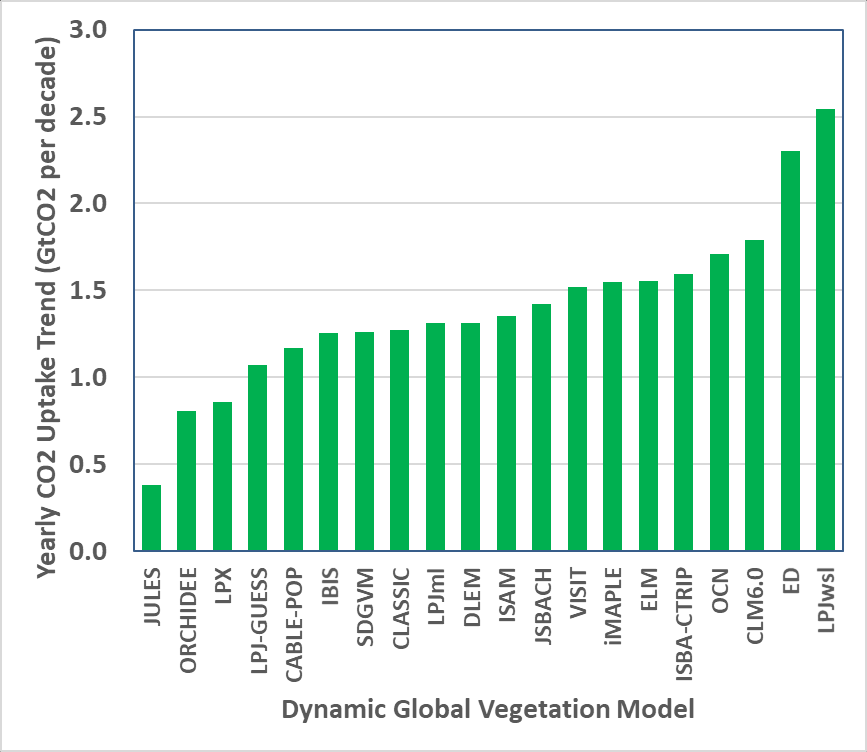
\includegraphics[width=1.0\textwidth]{bilder/bilderKlima-0013.png}\\[1cm]
\end{center}
\caption{Trends der jährlichen CO2-Aufnahme (GtCO2 pro Jahr und Jahrzehnt) durch Landprozesse
im Zeitraum 1959–2023, simuliert durch 20 verschiedene dynamische globale Vegetationsmodelle, die regelmäßig
vom Global Carbon Project (Friedlingstein, 2024) veröffentlicht werden.}
\end{figure}

\subsubsection*{CO$_2$-Aufnahme durch Landprozesse}
Die Aufnahme von zusätzlichem CO$_2$ aus der Atmosphäre durch Landoberflächenprozesse (wie auch aus der globalen Ergrünung geschlossen) wurde mit 20 verschiedenen dynamischen globalen Vegetationsmodellen modelliert, deren Ausgaben jährlich vom Global Carbon Project aktualisiert werden (Friedlingstein, 2024). Wie in Abb. 3.2.3 zu sehen ist, stimmen alle diese Modelle darin überein, dass Vegetation und Böden Kohlenstoff aus der Atmosphäre sequestriert haben. Aber wir sehen auch, dass die langfristigen Trends über 1959 bis 2023 (65 Jahre) stark zwischen den Modellen variieren, um fast einen Faktor von 7. Dies zeigt, dass erhebliche Unsicherheit darüber besteht, wie schnell Landprozesse CO$_2$ aus der Atmosphäre entfernen, was wiederum Unsicherheit in zukünftigen atmosphärischen CO$_2$-Konzentrationen schafft, die dann Unsicherheit in Klimamodellsimulationen zukünftiger Klimaveränderungen erzeugen.

\subsubsection*{CO$_2$-Aufnahme durch Ozeanprozesse}
Die Aufnahme von zusätzlichem CO$_2$ aus der Atmosphäre durch Ozeanprozesse wurde mit 10 verschiedenen Ozeanbiogeochemie-Modellen modelliert, deren Ausgaben jährlich vom Global Carbon Project aktualisiert werden (Friedlingstein, 2024). Wie die Ergebnisse der Landmodelle stimmen alle Ozeanmodelle darin überein, dass die globalen Ozeane während 1959-2023 Kohlenstoff aus der Atmosphäre mit einer steigenden Rate sequestriert haben (Abb. 3.2.4). Im Gegensatz zu den Landmodellen zeigen die Ozeanmodelle jedoch eine viel bessere Übereinstimmung miteinander, wobei das Modell mit der schnellsten steigenden CO$_2$-Aufnahme nur 65 Prozent schneller ist als das Modell mit der langsamsten steigenden CO$_2$-Aufnahme. Trotz der relativen Übereinstimmung zwischen den Modellen bemerkt Friedlingstein et al. (2022), dass es erhebliche Diskrepanzen zwischen den verschiedenen Methoden über die Stärke der Ozeansenke im letzten Jahrzehnt gibt, besonders im Südozean.
Beachten Sie, dass der durchschnittliche Trend in der CO$_2$-Aufnahme über alle Landmodelle in Abb. 3.2.3 25 Prozent größer ist als der durchschnittliche Trend in der Ozeanaufnahme. Dies deutet darauf hin, dass Landprozesse in ihrer Fähigkeit, CO$_2$ zu entfernen, schneller zunehmen als Ozeanprozesse ihre CO$_2$-Sequestrierung steigern.

\begin{figure}[H]
\begin{center}
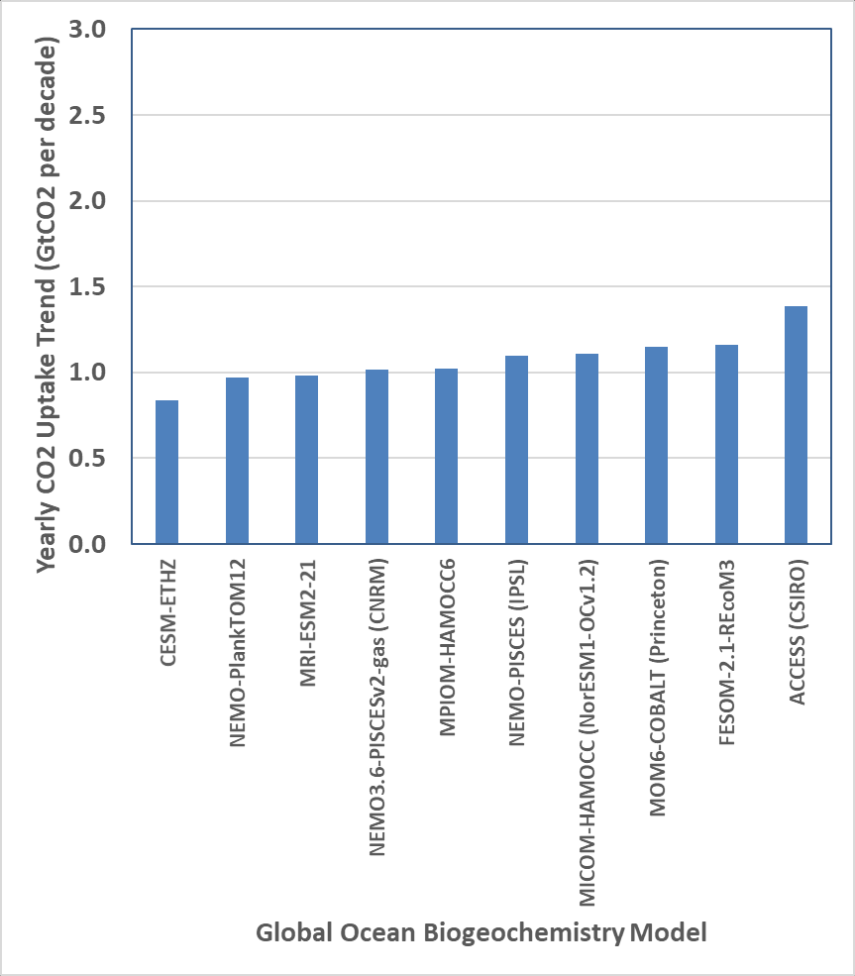
\includegraphics[width=1.0\textwidth]{bilder/bilderKlima-0015.png}\\[1cm]
\end{center}
\caption{Trends der jährlichen CO2-Aufnahme (GtCO2 pro Jahr und Jahrzehnt) durch Ozeanprozesse im Zeitraum
1959–2023, simuliert durch 10 verschiedene ozeanische Biogeochemie-Modelle, regelmäßig berichtet vom
Global Carbon Project (Friedlingstein, 2024).}
\end{figure}


\section{Urbanisierungseinfluss auf Temperaturtrends}
Historische Temperaturdaten über Land wurden hauptsächlich dort gesammelt, wo Menschen leben. Dies wirft das Problem auf, wie man nicht-klimatische Erwärmungssignale aufgrund von städtischen Wärmeinseln (UHI) und anderen Veränderungen der Landoberfläche herausfiltern kann. Wenn diese nicht entfernt werden, könnten die Daten beobachtete Erwärmung übermäßig Treibhausgasen zuschreiben. Das IPCC erkennt an, dass Rohtemperaturdaten mit UHI-Effekten kontaminiert sind, behauptet aber, Datenbereinigungsverfahren zu haben, die sie entfernen. Es ist eine offene Frage, ob diese Verfahren ausreichend sind.
AR6 spielte dieses Problem herunter, indem es sagte (WGI S. 235), dass keine neuen Beweise aufgetaucht seien, um die AR5-Feststellung zu ändern, dass Urbanisierung eine Aufwärtsverzerrung von nicht mehr als 10 Prozent im globalen Landerwärmungstrend verursacht. AR5 (WGI S. 189) zitierte ebenfalls die 10-Prozent-Obergrenze ohne Quellenangabe. AR4 (WGI S. 244) zitierte Jones et al. (1990) und Peterson et al. (1999) als Grundlage der Behauptung. Peterson et al. fanden keinen Unterschied in Trends zwischen ländlichen und städtischen Stichproben, obwohl ihre Definition von ländlich lokale Bevölkerungen bis zu 10.000 Personen einschloss, während der relative Einfluss der Urbanisierung deutlich darunter beginnt (Spencer et al., 2025). Jones et al. verglichen ländliche/städtische Erwärmung in drei Regionen: Ostaustralien, Ostchina und Westliche Sowjetunion. Ihre Definition von \emph{ländlich} umfasste Städte bis zu 10.000 in der ehemaligen Sowjetunion und bis zu 100.000 in China. Sie fanden relative Erwärmungsverzerrungen größer als 10 Prozent in diesen Gebieten, vermuteten aber, dass der Urbanisierungseffekt, gemittelt über die Gebiete, die sie nicht untersuchten, die globale Landverzerrung auf unter 10 Prozent des beobachteten Erwärmungstrends bringen würde.

Mehrere Arbeiten erschienen vor dem IPCC AR4, die argumentierten, dass der erwärmende Effekt von UHIs eine relativ große (30-50\%) Komponente zur beobachteten Erwärmung hinzufügte und nicht von Klimamodellen simuliert wurde (de Laat und Maurellis 2006, McKitrick und Michaels 2007). Diese Befunde basierten auf Korrelationen zwischen Orten maximaler Erwärmung über Land und Orten maximaler sozioökonomischer Entwicklung. AR4 behauptete (S. 244), dass diese Korrelationen ein Artefakt natürlicher atmosphärischer Zirkulationen waren und tatsächlich statistisch insignifikant, und verwarf die Befunde auf dieser Grundlage. Ihre Behauptung war kontrovers, weil sie ohne unterstützende Beweise präsentiert wurde. McKitrick (2010) und McKitrick und Nierenberg (2010) zeigten, dass die Berücksichtigung verschiedener vermuteter alternativer Erklärungen für die Korrelationen ihre Signifikanz nicht beeinflusste. AR5 (S. 189) räumte ein, dass AR4 \emph{keine expliziten Beweise} für seine Bewertung geliefert hatte und erkannte weiter auf der Grundlage dieser Arbeiten an, dass es \emph{signifikante Beweise für eine solche Kontamination der Aufzeichnung} gab, d.h. eine Erwärmungsverzerrung in der Landaufzeichnung. Wie bereits bemerkt, trugen sie jedoch an anderer Stelle im AR5-Bericht die AR4-Behauptung vor, dass es weniger als 10 Prozent der beobachteten Erwärmung seien. Außerdem gaben sie keine Warnung über die Verwendung der Landaufzeichnung für Klimamessungen, obwohl sie die Beweise für UHI-Kontamination einräumten. Kürzlich schätzten Soon et al. (2023) eine Urbanisierungsverzerrung in der nordhemisphärischen Landaufzeichnung über 1850-2018, die ausreicht, um den Trend in der gemischten Aufzeichnung von \SI{0.55}{\celsius} auf \SI{0.89}{\celsius} pro Jahrhundert zu erhöhen.

Einige Studien, die Beweise gegen UHI-Kontamination lieferten, verglichen Erwärmungsraten zwischen ländlichen und städtischen Standorten (Jones et al. 1990, Peterson et al. 1999, Wickham et al. 2013). Es ist nicht bekannt, ob solche Methoden UHI-Verzerrung erkennen könnten, selbst wenn sie vorhanden wäre. Der Einfluss der UHI-Erwärmung ist logarithmisch in der Bevölkerung, mit anderen Worten, er ist am stärksten bei niedriger Bevölkerungsdichte und flacht dann ab, wenn sich die lokale Urbanisierung ausdehnt (Oke 1973, Spencer et al. 2025). Daher beweist das Versagen, einen Unterschied in Erwärmungsraten zwischen städtischen und ländlichen Stationen zu finden, nicht die Abwesenheit von UHI-Kontamination. McKitrick (2013) lieferte eine empirische Demonstration, in der sich die ländlichen/städtischen Trends in einem Datensatz, der aus anderen Gründen als mit UHI-Verzerrung kontaminiert erwiesen wurde, nicht signifikant unterschieden.

Parker (2006) untersuchte eine Stichprobe städtischer Standorte und fand keinen Unterschied in Trends zwischen Untergruppen, die nach nächtlicher Windgeschwindigkeit unterteilt waren, und schloss auf dieser Grundlage, dass Urbanisierung kein signifikanter Faktor sein könnte. Auch hier ist die Frage, ob eine solche Methode UHI-Verzerrung finden würde, selbst wenn sie vorhanden wäre. McKitrick (2013) präsentierte ein Beispiel, in dem UHI-kontaminierte Daten keine signifikanten Trendunterschiede zeigten, wenn sie nach Windgeschwindigkeit stratifiziert wurden.

Die Herausforderung bei der Messung von UHI-Verzerrung besteht darin, lokale Temperaturveränderungen mit einer entsprechenden Veränderung in Bevölkerung oder Urbanisierung zu verknüpfen, anstatt mit einer statischen Klassifikationsvariable wie ländlich oder städtisch. Spencer et al. (2025) verwendeten neu verfügbare historische Bevölkerungsarchive, um eine solche Analyse durchzuführen, und fanden Beweise für signifikante UHI-Verzerrung in US-Sommertemperaturdaten.

Zusammenfassend, während es eindeutig Erwärmung in der Landaufzeichnung gibt, gibt es auch Beweise dafür, dass sie durch Urbanisierungsmuster nach oben verzerrt ist und dass diese Verzerrungen nicht vollständig durch die Datenverarbeitungsalgorithmen entfernt wurden, die zur Erstellung von Klimadatensätzen verwendet werden.

\vfill
{\textbf Literaturverzeichnis:}

Angert, A., S. Biraud, Bonfils, C., Buermann, W. and I. Fung (2004). CO2 seasonality indicates origins of
post-Pinatubo sink. Geophysical Research Letters 31. \url{https://doi.org/10.1029/2004GL019760}

AR6: Intergovernmental Panel on Climate Change Sixth Assessment Report (2021) Working Group I
Contribution. www.ipcc.ch.

AR5: Intergovernmental Panel on Climate Change Fifth Assessment Report (2013) Working Group I
Contribution. www.ipcc.ch.

AR4: Intergovernmental Panel on Climate Change Fourth Assessment Report (2007) Working Group I
Contribution. www.ipcc.ch.

Burgess, Matthew et al (2021) Environmental Research Letters 16 014016
\url{}

Ciais, P., C. Sabine, G. Bala, L. Bopp, V. Brovkin,et al. (2013): Carbon and Other Biogeochemical Cycles.
In: Climate Change 2013: The Physical Science Basis. Contribution of Working Group I to the Fifth
Assessment Report of the Intergovernmental Panel on Climate Change [Stocker, T.F., D. Qin, G.-K.
Plattner, M. Tignor,et al. (eds.)]. Cambridge University Press, Cambridge, United Kingdom and New
York, NY, USA

Connolly, Roman, Willie Soon, Michael Connolly et al. (2021) How much has the Sun influenced
Northern Hemisphere temperature trends? An ongoing debate Research in Astronomy and
Astrophysics 21(6) doi: 10.1088/1674-4527/21/6/131 \url{https://iopscience.iop.org/article/10.1088/1674-
4527/21/6/131}

Crisp, David \& Dolman, Han (A.J.) \& Tanhua, Toste \& Mckinley, Galen \& Hauck, Judith \& Bastos, Ana
\& Sitch, Stephen \& Eggleston, Simon \& Aich, Valentin. (2022). How Well Do We Understand the
Land‐Ocean‐Atmosphere Carbon Cycle?. Reviews of Geophysics. 60. 10.1029/2021RG000736.

De Laat, A.T.J., and A.N. Maurellis (2006), Evidence for influence of anthropogenic surface processes on
lower tropospheric and surface temperature trends, International Journal of Climatology 26:897—913.

Friedlingstein, P., and 95 co-authors (2024): Global Carbon Budget 2024, Earth System Science Data
14(4), https://essd.copernicus.org/preprints/essd-2024-519

Hausfather et al. (2019) “Evaluating the Performance of Past Climate Model Projections” Geophysical
Research Letters 47(1) https://doi.org/10.1029/2019GL085378

Hausfather, Z. and G. Peters (2020a) “Emissions – the ‘business as usual’ story is misleading” Nature 29
January 2020 https://www.nature.com/articles/d41586-020-00177-3

Hausfather, Z. and G. Peters (2020b) RCP8.5 is a problematic scenario for near-term emissions.
Proceedings of the National. Academy of Sciences 117, 27791–27792 (2020)

Jenkins, S., Smith, C., Allen, M. et al. Tonga eruption increases chance of temporary surface temperature
anomaly above 1.5 °C. Nature Climate Change. 13, 127–129 (2023). https://doi.org/10.1038/s41558-
022-01568-2

Jones, P. D., P. Y. Groisman, M. Coughlan, N. Plummer, W.-C. Wang, and T. R. Karl (1990),
Assessment of urbanization effects in time series of surface air temperature over land, Nature, 347,
169 – 172

Liu, Pengfei et al. (2021) “Improved estimates of preindustrial biomass burning reduce the magnitude of
aerosol climate forcing in the Southern Hemisphere” Science Advances 7(22) May 2021
https://doi.org/10.1126/sciadv.abc1379

McKitrick, R.R. and P.J. Michaels (2007), Quantifying the influence of anthropogenic surface processes
and inhomogeneities on gridded global climate data, Journal of Geophysical Research, 112, D24S09,
doi:10.1029/2007JD008465.

McKitrick, Ross R. (2010) Atmospheric Oscillations Do Not Explain the Temperature-Industrialization
Correlation. Statistics Politics and Policy Vol 1. No. 1., July 2010

McKitrick, Ross R. (2013) Encompassing Tests of Socioeconomic Signals in Surface Climate
Data. Climatic Change doi 10.1007/s10584-013-0793-5. Volume 120, Issue 1-2.
http://link.springer.com/article/10.1007%2Fs10584-013-0793-5

McKitrick, Ross R. and Nicolas Nierenberg (2010) Socioeconomic Patterns in Climate Data. Journal of
Economic and Social Measurement, 35(3,4) pp. 149-175. DOI 10.3233/JEM-2010-0336

McKitrick, Ross R., Mark Strazicich and Junsoo Lee (2012) “Long-Term Forecasting of Global Carbon
Dioxide Emissions: Reducing Uncertainties Using a Per-Capita Approach.” Journal of
Forecasting, Vol 32, Issue 5, pp 435-451 DOI: 10.1002/for.2248.

Oke, T.R., 1973: City size and the urban heat island, Atmospheric Environment 7, 769-77922

Parker, D.E. (2006) “A Demonstration that Large-Scale Warming is not Urban.” Journal of Climate
19:2882—2895.

Peterson, Thomas C., Kevin P. Gallo, Jay Lawrimore, Timothy W. Owen, Alex Huang, David A.
McKittrick (1999) Global rural temperature trends. Geophysical Research Letters February 1999
https://doi.org/10.1029/1998GL900322

Pielke Jr., Roger and Ritchie, Justin (2020) “Systemic Misuse of Scenarios in Climate Research and
Assessment” Social Sciences Research Network April 2020, available at:
https://ssrn.com/abstract=3581777

Pielke Jr, R., Burgess, M. G., \& Ritchie, J. (2022). Plausible 2005-2050 emissions scenarios project
between 2 and 3 degrees C of warming by 2100. Environmental Research Letters 17 024027
https://iopscience.iop.org/article/10.1088/1748-9326/ac4ebf/pdf

Scaffeta, Nicola, Richard C. Willson, Jae N. Lee and Dong Wu (2019) Modeling Quiet Solar Luminosity
Variability from TSI Satellite Measurements and Proxy Models during 1980–2018. Remote Sensing
11(21) 2569 https://doi.org/10.3390/rs11212569

Schoeberl, M.R., Y. Wang, G. Taha, D.J. Zawada, R. Ueyama and A. Dessler, 2024. Evolution of the
climate forcing during the two years after the Hunga Tonga-Hunga Ha’apai eruption. Journal of
Geophysical Research., 129.

Schwalm, C.R., S. Glendon, P. B. Duffy (2020) RCP8.5 tracks cumulative CO2 emissions. Proceedings of
the National Academy of Sciences U.S.A. 117, 19656–19657 (2020).

Soon,W.; Connolly, R.; Connolly, M.; Akasofu, S.-I.; Baliunas, S.; et al. (2023) The Detection and
Attribution of Northern Hemisphere Land Surface Warming (1850–2018) in Terms of Human and
Natural Factors: Challenges of Inadequate Data. Climate 2023, 11, 179.
https://doi.org/10.3390/cli11090179

Spencer, Roy W, John R Christy and William D. Braswell (2025) Urban Heat Island Effects in U.S.
Summer Surface Temperature Data, 1895–2023 Journal of Applied Meteorology and Climatology
April 2025 https://doi.org/10.1175/JAMC-D-23-0199.1

Wickham C, R Rohde , RA Muller, J Wurtele, J Curry, et al. (2013) Influence of Urban Heating on the
Global Temperature Land Average using Rural Sites Identified from MODIS Classifications.
Geoinformatics and Geostatistics: An Overview 1:2.

Zacharias, Pia (2014) An Independent Review of Existing Total Solar Irradiance Records. Surveys in
Geophysics 35 pp. 897—912 https://link.springer.com/article/10.1007/s10712-014-9294-y

\cleardoublepage
\chapter*{TEIL II: KLIMAREAKTION AUF CO$_2$-EMISSIONEN}
%\numberwithin{figure}{chapter}
\FigureNumbersByChapter
\addcontentsline{toc}{chapter}{TEIL II: KLIMAREAKTION AUF CO$_2$-EMISSIONEN}
\cleardoublepage
\chapter{Klimasensitivität bezüglich CO$_2$-Einwirkung}
\paragraph{Kapitelzusammenfassung}
\begin{quote}
Es gibt eine wachsende Erkenntnis, dass Klimamodelle nicht für den Zweck geeignet sind, die Gleichgewichts-Klimasensitivität (ECS) des Klimas gegenüber steigendem CO$_2$ zu bestimmen. Das IPCC hat sich datengetriebenen Ansätzen zugewandt, einschließlich historischer Daten und paläoklimatischer Rekonstruktionen, aber deren Zuverlässigkeit ist durch Datenmängel beeinträchtigt.
Datengetriebene ECS-Schätzungen tendieren dazu, niedriger zu sein als klimamodell-generierte Werte. Die obere Grenze des IPCC AR6 für den wahrscheinlichen ECS-Bereich beträgt \SI{4.0}{\celsius}, niedriger als der AR5-Wert von \SI{4.5}{\celsius}. Diese Senkung der oberen Grenze scheint durch paläoklimatische Daten gut begründet zu sein. Die untere Grenze des AR6 für den wahrscheinlichen ECS-Bereich beträgt \SI{2.5}{\celsius}, wesentlich höher als der AR5-Wert von \SI{1.5}{\celsius}. Diese Erhöhung der unteren Grenze ist weniger gerechtfertigt; Belege seit AR6 zeigen, dass die untere Grenze des wahrscheinlichen Bereichs bei etwa \SI{1.8}{\celsius} liegt.
\end{quote}
\section{Einführung}
Das Ausmaß der Klimareaktion auf steigende CO$_2$-Konzentrationen steht im Zentrum der wissenschaftlichen Debatte über den anthropogenen Klimawandel und damit auch der öffentlichen Debatte über \emph{Klimaschutzmaßnahmen}. Das einfachste Maß für diese Reaktion ist der Anstieg der globalen durchschnittlichen Oberflächentemperatur, quantifiziert durch die Gleichgewichts-Klimasensitivität (ECS). ECS ist definiert als das Ausmaß der Erwärmung, das als Reaktion auf eine Verdoppelung von CO$_2$ von seiner vorindustriellen Konzentration von \SI{280}{ppm} erwartet wird, nachdem alle Klimakomponenten Zeit hatten, sich anzupassen. Einige Komponenten, wie die Temperaturen in der unteren Atmosphäre (Troposphäre), passen sich schnell an, während andere wie der tiefe Ozean und die Kryosphäre möglicherweise jahrhundertelang brauchen. Ein verwandtes Maß, die Transiente Klimareaktion (TCR), beschreibt die kürzeren Zeitskalen besser; sie ist definiert als das Ausmaß der Erwärmung, wenn die CO$_2$-Konzentration durch einen jährlichen Anstieg von einem Prozent über 70 Jahre verdoppelt wird.

Der Charney-Bericht von 1979 für die U.S. National Academy of Sciences (National Research Council 1979) schlug vor, dass die wahrscheinlichste ECS \SI{3.0}{\celsius} $±$ \SI{1.5}{\celsius} sei. Das IPCC bekräftigte diesen Bereich wiederholt mit nur geringfügigen Variationen bis zu seinem jüngsten AR6. AR5 bezeichnete \SIrange{1.5}{4.5}{\celsius} als den wahrscheinlichen Bereich (66 Prozent Wahrscheinlichkeit) und stellte fest, dass ECS extrem unwahrscheinlich (95 Prozent Wahrscheinlichkeit) unter \SI{1.0}{\celsius} und sehr unwahrscheinlich (90 Prozent Wahrscheinlichkeit) über \SI{6.5}{\celsius} liegt.

Die Unsicherheit in ECS ist hartnäckig weit geblieben, trotz vieler einzelner Studien, die behaupteten, sie zu verringern (Hausfather 2023). Zuletzt verengte AR6 den wahrscheinlichen Bereich auf \SIrange{2.5}{4.0}{\celsius} und betrachtete den sehr wahrscheinlichen Bereich als \SIrange{2.0}{5.0}{\celsius}. Diese Verengung am unteren Ende wird bestritten, wie unten diskutiert wird.

Unsicherheiten in ECS sind höchst folgenreich für die Politikgestaltung. Wie in Kapitel 11 diskutiert wird, verwenden Wirtschaftsmodelle ECS-Werte, um die Kosten von CO$_2$-Emissionen zu projizieren. Der traditionelle Wert (\SI{3.0}{\celsius}) hat typischerweise bescheidene globale soziale Kosten von CO$_2$-Emissionen ergeben, ausreichend um einige politische Maßnahmen zu rechtfertigen, aber meist auf später in diesem Jahrhundert verschoben. Wenn ECS sehr hoch ist (über \SI{4.5}{\celsius}), werden sofortige aggressive Emissionskontrollen zwingender, während keine CO$_2$-Emissionskontrollen wirtschaftlich gerechtfertigt sind für ECS unter \SI{2.0}{\celsius} (Dayaratna et al. 2017, 2020). Eine präzise Schätzung zu erhalten ist unmöglich, daher muss die Politikgestaltung die Unsicherheit berücksichtigen.

Für sich allein ist der Gleichgewichts-Erwärmungseffekt einer Verdoppelung des atmosphärischen CO$_2$ etwas mehr als \SI{1}{\celsius} (Soden und Held 2006). Größere Werte von ECS entstehen durch positive Rückkopplungen, die die CO$_2$-Erwärmung verstärken. Wasserdampf-Rückkopplung ist positiv: eine wärmere Atmosphäre könnte mehr Wasserdampf haben, der selbst ein starkes Treibhausgas ist. Wärmere Temperaturen führen auch zu weniger Schnee- und Meereisbedeckung, wodurch die Erde mehr von der Sonnenstrahlung absorbieren kann. Einige einfache Schätzungen dieser Rückkopplungen erhöhen die ECS auf etwa \SI{2}{\celsius} (Sherwood et al., 2020). Größere Werte von ECS sind mit positiven Wolken-Rückkopplungen verbunden.

Klimawissenschaftler verwenden mehrere Beweislinien, um die Gleichgewichts-Klima\-sensitivität zu bestimmen:
\begin{itemize}
\item  Klimamodell-Simulationen
\item  Historische Beobachtungen  
\item  Paläoklimatische Rekonstruktionen
\item  Prozessverständnis von Rückkopplungen
\end{itemize}

\section{Modellbasierte Schätzungen der Klimasensitivität}
Die in IPCC AR4 und AR5 angegebenen ECS-Bereiche wurden hauptsächlich durch die Untersuchung des Verhaltens großmaßstäblicher Klimamodelle, auch General Circulation Models (GCMs) genannt, erhalten. Das IPCC änderte jedoch den Kurs in seinem AR6, als es sich einer direkteren datengetriebenen Methodik zuwandte. Hier diskutieren wir einige der Fallstricke bei der Verwendung von GCMs, um die Klimasensitivität der Erde zu bestimmen.

ECS kann aus Klimamodell-Simulationen bestimmt werden, indem die CO$_2$-Konzentration verdoppelt und mehrere Jahrhunderte für die Erwärmung zum Gleichgewicht ermöglicht werden. Um die Notwendigkeit solch langer Simulationen zu vermeiden, wird \emph{effektive Klimasensitivität} üblicherweise aus einer 150-Jahres-Simulation als Reaktion auf eine plötzliche Vervierfachung von CO$_2$ bewertet.

Im Prinzip ist ECS eine emergente Eigenschaft von GCMs –- das heißt, sie wird nicht direkt parametrisiert oder abgestimmt, sondern entsteht vielmehr in den Ergebnissen der Simulation. Anderweitig plausible GCMs und Parameterauswahlen wurden verworfen wegen wahrgenommener Konflikte mit einer erwarteten Erwärmungsrate oder Abneigung gegen eine Klimasensitivität des Modells außerhalb eines akzeptierten Bereichs (Mauritsen et al. 2012). Diese Praxis war für die in AR4 verwendeten Modelle üblich; Modellierer sind mit der Zeit von dieser Praxis abgekommen. Jedoch, selbst in einem CMIP6-Modell, stellen Mauritsen und Roeckner (2020) das Folgende bezüglich ihres Max-Planck-Institut (MPI) Klimamodells fest (Hervorhebung hinzugefügt):

\begin{quote}
Wir haben dokumentiert, wie wir das globale Klimamodell MPI-ESM1.2 abstimmten, um der instrumentellen Aufzeichnung der Erwärmung zu entsprechen; ein Unterfangen, das eindeutig erfolgreich war. Aufgrund der historischen Reihenfolge der Ereignisse war die Wahl, dies praktisch zu tun, indem eine ECS von etwa 3 K mittels Wolken-Rückkopplungen anvisiert wurde, anstatt die Aerosol-Forcierung abzustimmen.  
\end{quote}

Mit anderen Worten, die MPI-Modellierer wählten einen ECS-Wert von \SI{3}{\celsius} und stimmten dann die Wolken-Parametrisierungen ab, um ihr beabsichtigtes Ergebnis zu erreichen.

Wie bemerkt, ist die direkte Erwärmung durch CO$_2$-Verdoppelung nur etwa \SI{1}{\celsius} (Soden und Held 2006); weitere Erwärmung entsteht durch Klima-Rückkopplungen, die nicht explizit vom GCM aufgelöst werden, sondern auf Parametrisierungen physikalischer Prozesse angewiesen sind. Höhere Werte von ECS entstehen primär durch positive Wolken-Rückkopplungen, während das Ausmaß und sogar das Vorzeichen der Rückkopplungen sehr unsicher sind. Elemente der Wolken-Rückkopplung umfassen Änderungen in der Breitenverteilung von Wolken, Änderungen in der Verteilung der Wolkenhöhe (Änderungen in niedrigen versus hohen Wolken), Änderungen in der Phase von Wolken (Eis versus Flüssigkeit), Änderungen in der Wolkenpartikelgröße (verbunden mit Änderungen in Konzentration und/oder Zusammensetzung von Aerosolpartikeln), Änderungen in der Niederschlagseffizienz von Wolken, und sogar Änderungen darin, wie Wolken über den täglichen Sonnenzyklus verteilt sind (Curry und Webster, 1999). Es ist für GCMs schwierig, irgendeinen dieser Prozesse aufgrund ihrer kleinen Skala korrekt zu simulieren, geschweige denn vorherzusagen, wie sie sich in der Zukunft ändern werden. Weiterhin modulieren Wolkenprozesse die Größenordnungen der Wasserdampf-, Lapse-Rate- und Oberflächenalbedo-Rückkopplungen.

\begin{figure}[H]
\begin{center}
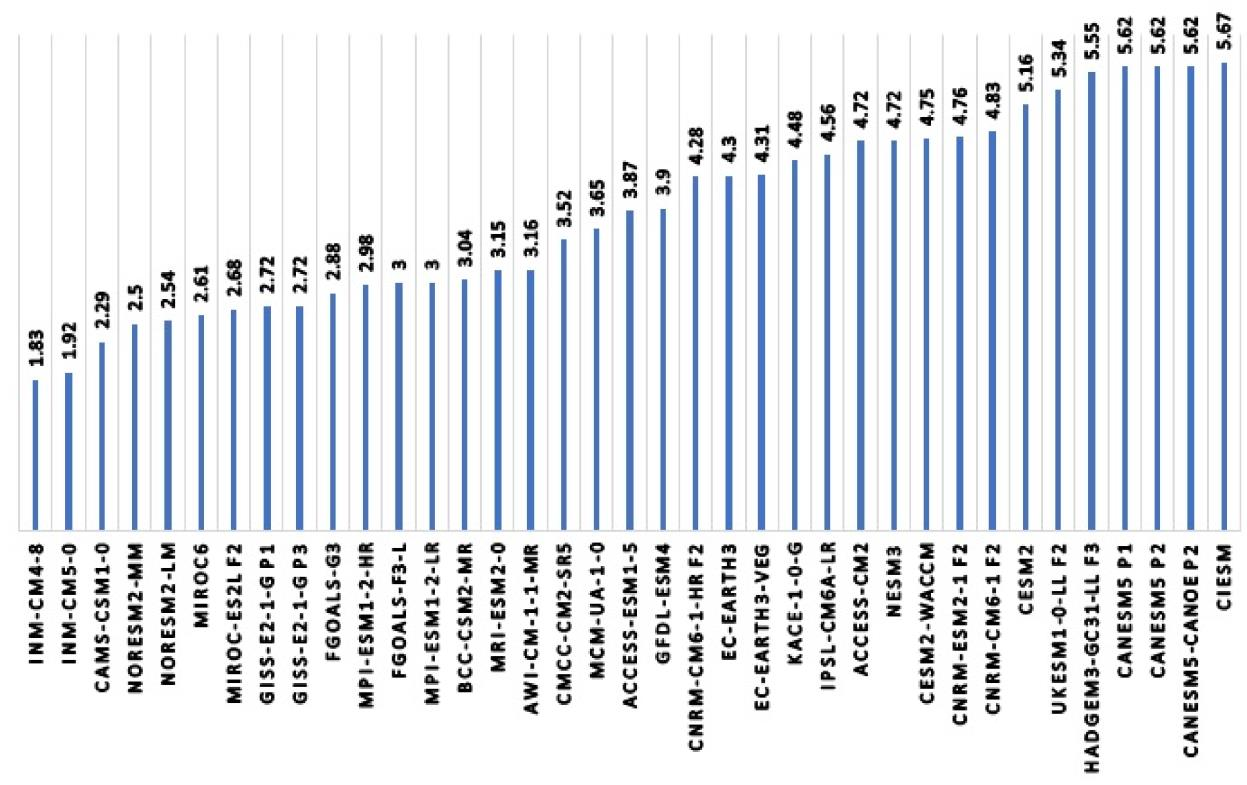
\includegraphics[width=1.0\textwidth]{bilder/bilderKlima-0017.jpg}\\[1cm]
\end{center}
\caption{Gleichgewichtsklimasensitivitäten in °C von 37 Klimamodellen aus dem CMIP6-Ensemble.
Die Kennungen für die verschiedenen Modelle sind auf der horizontalen Achse angegeben. Aus (Scafetta, 2021)}
\end{figure}


Die Spannweite der ECS-Werte aus dem CMIP5-Ensemble von Klimamodellen, die in AR5 verwendet wurden, war \SIrange{2.0}{4.7}{\celsius}; dieser Bereich vergrößerte sich für die CMIP6-Modelle, die in AR6 verwendet wurden, auf zwischen $1.8$ und \SI{5.7}{\celsius} (Chen et al., 2021, Scaffeta 2021, siehe Abbildung 4.1). Weit davon entfernt, die modellbasierte Klimasensitivität aufzulösen, scheint sich der Bereich zu vergrößern. Die Hauptursache der gesamten Aufwärtsverschiebung in ECS in CMIP6 relativ zu CMIP5 ist eine größere positive Wolken-Rückkopplung, angetrieben durch Änderungen in den Wolken-Parametrisierungen in vielen CMIP6-Modellen (Zelinka et al., 2020).

Aufgrund von Bedenken über Modellabstimmung und die hohe Empfindlichkeit gegenüber Wolken-Parametrisierungen stützte sich AR6 (2021) nicht auf Klimamodell-Simulationen in ihrer Bewertung der Klimasensitivität, sondern verließ sich stattdessen auf datengetriebene Methoden.

\section{Datengetriebene Schätzungen der Klimasensitivität}
Klimasensitivität kann auch aus instrumentellen Aufzeichnungen von Oberflächentemperaturen und ozeanischem Wärmeinhalt geschätzt werden, kombiniert mit Schätzungen darüber, wie sich Klimaforcierungen (z.B. Treibhausgase, solar, Vulkane, Aerosole) in der Vergangenheit verändert haben (Otto et al., 2013). Mit dieser Information kann ein einfaches empirisches Energiebilanz-Modell eingesetzt werden. Es erfordert die Schätzung eines Rückkopplungsparameters, dessen Unsicherheiten in der resultierenden ECS stark verstärkt werden (Roe und Baker, 2007).

Die Genauigkeit der datengetriebenen Methoden hängt von der Qualität der Eingangsdaten ab. Annahmen sind über ozeanische Wärmespeicherung nötig, und gute Daten sind nur für die letzten Jahrzehnte verfügbar. Die größte Quelle der Unsicherheit ist die Menge und Zusammensetzung von Aerosolpartikeln und ihre Wechselwirkungen mit Wolkenstrahlungseigenschaften (der sogenannte indirekte Aerosoleffekt; siehe Abbildungen 3.1.1, 3.1.2). Klimamodelle zeigen Erwärmung als Reaktion auf THG, aber Abkühlung als Reaktion auf Aerosole (Schwartz et al., 2007). Beobachtete Erwärmung des 20. Jahrhunderts kann gezeigt werden, dass sie konsistent ist entweder mit niedriger ECS und niedriger Aerosol-Abkühlung, oder hoher ECS und hoher Aerosol-Abkühlung. Da die Verwendung fossiler Brennstoffe sowohl THG als auch Aerosole zur Atmosphäre hinzufügt, müssen beide Effekte geschätzt werden, um den Erwärmungseffekt von CO$_2$ zu isolieren.

Paläoklima-Proxies werden auch verwendet, um die Sensitivität vergangener Klimate zu bewerten, indem paläoklimatische Änderungen in den Erdtemperaturen mit Schätzungen von Änderungen in Forcierungen verglichen werden. Die zwei informativsten Perioden sind das letzte glaziale Maximum (vor etwa 20.000 Jahren), das etwa \SIrange{3}{7}{\celsius} kälter war als heute, und eine mittlere Pliozän-Periode (vor etwa drei Millionen Jahren), die \SIrange{1}{3}{\celsius} wärmer war als heute. Die Grenzen der Abkühlung während des letzten glazialen Maximums geben den besten einzelnen Beweis, dass hohe Werte der Klimasensitivität unwahrscheinlich sind. Jedoch sind paläoklimatische Schätzungen mit sehr großen Unsicherheiten in den geschätzten Temperaturen und Forcierungen verbunden. Weiterhin könnten Schätzungen der Klimasensitivität basierend auf vergangenen Klimazuständen nicht auf den aktuellen Zustand des Klimasystems anwendbar sein.

Ein wiederkehrendes Thema in der Klimaliteratur ist, dass ECS-Schätzungen basierend auf historischen Daten kleiner sind als ECS-Schätzungen, die aus Klimamodellen abgeleitet werden (Sherwood und Forest 2024). Etwa 15 Schätzungen basierend auf historischen Daten erschienen in der begutachteten Literatur zwischen 2012 und 2024, die ECS-Bestschätzungen zwischen \SI{1.0}{\celsius} und \SI{2.5}{\celsius} ergaben, obwohl Kritiker einige der Methoden und die Datenqualität in Frage gestellt haben. Für AR6 legte das IPCC primäres Gewicht auf die Ergebnisse von Sherwood et al. (2020), die historische Daten und paläoklimatische Proxies mit dem prozessbasierten Ansatz kombinierten und eine Bestschätzung von \SI{3.1}{\celsius} mit einem wahrscheinlichen Bereich von \SIrange{2.6}{3.9}{\celsius} ergaben. Lewis (2022) äußerte eine Reihe von Bedenken über dieses Ergebnis, einschließlich methodologischer Fehler, veralteter Eingangswerte und der Verwendung subjektiver Bayesscher Priors in der Analyse. Lewis' Analyse fand, dass Klimasensitivität geschätzt wird, viel niedriger und besser eingegrenzt zu sein als in der Sherwood et al. Analyse – Median \SI{2.2}{\celsius} (\SIrange{1.8}{2.7}{\celsius} im $17–83$ Prozent wahrscheinlichen Bereich, und \SIrange{1.6}{3.2}{\celsius} im $5–95$ Prozent sehr wahrscheinlichen Bereich). Das IPCC AR6 schätzte nur eine $5$ Prozent Wahrscheinlichkeit, dass ECS unter \SI{2.3}{\celsius} lag, während Lewis es auf über $50$ Prozent schätzte. Die jüngsten Veröffentlichungen in der Debatte zwischen Sherwood et al. und Lewis verteidigen weiterhin ihre jeweiligen Positionen: Sherwood und Foster (2024) und Lewis (2025).

Ein in AR6 betontes Argument ist, dass datengetriebene ECS-Schätzungen die zukünftige Erwärmungsreaktion auf THG unterschätzen könnten wegen eines sogenannten \emph{Mustereffekts} (Forster et al., 2021). Es wird geglaubt, dass der tropische Pazifik die Gesamteffizienz, mit der die Erde Wärme in den Weltraum abstrahlt, stark beeinflusst, aber einige Regionen entfernen Wärme effizienter als andere. Wenn der West-Ost-Temperaturgradient im tropischen Pazifik in einem sich erwärmenden Klima geschwächt wird, würde sich die Erwärmung dort konzentrieren, wo Wärme weniger effizient entfernt wird, was ECS erhöht.

Die meisten Klimamodelle simulieren, dass steigende THG den West-Ost-Temperatur\-gradienten schwächen werden, was das IPCC in AR6 zu dem Schluss führte, dass datengetriebene ECS-Schätzungen den zukünftigen ECS-Wert unterschätzten. Jedoch wiesen Seager et al. (2019) darauf hin, dass, entgegen den Modellen, sich der West-Ost-Temperaturgradient über die Zeit verstärkt hat. Sie argumentierten weiter, dass der Mechanismus, der anderes in Klimamodellen vorhersagt, auf einer fehlerhaften Charakterisierung ozeanischer Dynamik basierte und es keinen Grund gibt zu erwarten, dass sich der Gradient schwächt. Ein ähnliches Argument wurde kürzlich von Lee et al. (2024) gemacht, die schlossen, dass \emph{die Trajektorie des beobachteten Trends die Reaktion auf zunehmende THG-Belastung in der Atmosphäre widerspiegelt}; mit anderen Worten, THG-Erwärmung sollte zu einer zukünftigen Verstärkung statt einer Schwächung des Temperaturgradienten führen. Erhöhte Effizienz der atmosphärischen Abkühlung impliziert, wenn überhaupt, dass die zukünftige ECS in einem sich erwärmenden Klima niedriger sein könnte als aktuelle Schätzungen.

\section{Transiente Klimareaktion}
Die Transiente Klimareaktion (TCR) bietet eine nützlichere Beobachtungseinschränkung für die Klimasensitivität. TCR ist der globale Temperaturanstieg, der entsteht, wenn CO$_2$ mit einer jährlichen Rate von 1 Prozent über einen Zeitraum von 70 Jahren erhöht wird (d.h. allmählich verdoppelt). Im Vergleich zur ECS vermeiden beobachtungsbasiert bestimmte Werte von TCR die Probleme von Unsicherheiten in der ozeanischen Wärmeaufnahme und der unscharfen Grenze bei der Definition des Gleichgewichts, die aus einer Reihe von Zeitskalen für die längerfristigen Rückkopplungsprozesse (z.B. Eisschilde) entstehen. TCR ist durch historische Erwärmung besser eingegrenzt als ECS. AR6 beurteilte den sehr wahrscheinlichen Bereich von TCR als \SIrange{1.2}{2.4}{\celsius}. Im Gegensatz zu ECS ist die obere Grenze von TCR enger eingegrenzt. Zum Vergleich: die von Lewis (2023) bestimmten TCR-Werte liegen bei $1.25$ bis \SI{2.0}{\celsius}, was eine viel bessere Übereinstimmung mit AR6-Werten zeigt, als beim Vergleich der ECS-Werte zu sehen war.

\vfill
{\textbf Literaturverzeichnis:}

Carbon Brief. (2020, July 22). Explainer: How scientists estimate climate sensitivity.
https://www.carbonbrief.org/explainer-how-scientists-estimate-climate-sensitivity

Carbon Brief. (2020, July 22). Guest post: Why low-end ‘climate sensitivity’ can now be ruled out.
https://www.carbonbrief.org/guest-post-why-low-end-climate-sensitivity-can-now-be-ruled-out

Carbon Brief. (2021, August 9). In-depth Q\&A: The IPCC’s sixth assessment report on climate science.
https://www.carbonbrief.org/in-depth-qa-the-ipccs-sixth-assessment-report-on-climate-science

Chen, D., et al. (2021). Framing, context, and methods. In V. Masson-Delmotte et al. (Eds.), Climate
change 2021: The physical science basis. Contribution of Working Group I to the Sixth Assessment
Report of the Intergovernmental Panel on Climate Change. Cambridge University Press.

Curry, J. A., \& Webster, P. J. (1999). Thermodynamic feedbacks in the climate system. In
Thermodynamics of atmospheres and oceans (pp. 351–385). Academic Press.

Dayaratna, Kevin, Ross McKitrick and David Kreutzer (2017) Empirically-Constrained Climate Sensitivity
and the Social Cost of Carbon. Climate Change Economics April 2017 DOI:
http://dx.doi.org/10.1142/S2010007817500063

Dayaratna, Kevin, Ross McKitrick and Patrick J. Michaels (2020) Climate Sensitivity, Agricultural
Productivity and the Social Cost of Carbon in FUND. Environmental Economics and Policy Studies
https://doi.org/10.1007/s10018-020-00263-w

Forster, P., et al. (2021). The Earth's energy budget, climate feedbacks, and climate sensitivity. In V.
Masson-Delmotte et al. (Eds.), Climate change 2021: The physical science basis. Contribution of
Working Group I to the Sixth Assessment Report of the Intergovernmental Panel on Climate Change.
Cambridge University Press.

Hausfather, Z. (2020, July 22). Explainer: How scientists estimate climate sensitivity. Carbon Brief.
https://www.carbonbrief.org/explainer-how-scientists-estimate-climate-sensitivity

Lan, X., Tans, P., \& Thoning, K. W. (2025). Trends in globally-averaged CO$_2$ determined from NOAA
Global Monitoring Laboratory measurements. NOAA Global Monitoring Laboratory.
https://doi.org/10.15138/9N0H-ZH07

Lee, S., Byrne, M. P., Loikith, P. C., \& O’Dell, C. W. (2024). Zonal contrasts of the tropical Pacific
climate predicted by a global constraint. Climate Dynamics, 62(1–2), 229–246.
https://doi.org/10.1007/s00382-023-06741-7

Lewis, N. (2023). Objectively combining climate sensitivity evidence. Climate Dynamics, 61(9–10),
3155–3163. https://doi.org/10.1007/s00382-022-06398-8

Lewis, N. (2025). Comment on “Can uncertainty in climate sensitivity be narrowed further?” by
Sherwood and Forest (2024). EGUsphere [preprint]. https://doi.org/10.5194/egusphere-2025-1179

Thorsten Mauritsen et al., (2012) “Tuning the Climate of a Global Model,” Journal of Advances in
Modeling Earth Systems 4, no. 3 https://doi. org/10.1029/2012ms000154
29

Mauritsen, T., \& Roeckner, E. (2020). Tuning the MPI-ESM1.2 global climate model to improve the
match with instrumental record warming by lowering its climate sensitivity. Journal of Advances in
Modeling Earth Systems, 12, e2019MS002037. https://doi.org/10.1029/2019MS002037

Otto, A., Otto, F. E. L., Boucher, O., Church, J., Hegerl, G., Forster, P. M., Gregory, J. M., \& Johnson, G.
C. (2013). Energy budget constraints on climate response. Nature Geoscience, 6(6), 415–416.
https://doi.org/10.1038/ngeo1836

Pachauri, R. K., \& Meyer, L. (Eds.). (2015). Climate change 2014: Synthesis report. Intergovernmental
Panel on Climate Change.

Roe, G. and M. Baker (2007). Why is climate sensitivity so unpredictable? Science 318, 629-632.
https://doi.org/10.1126/science.1144735

Scafetta, N. (2021). Testing the CMIP6 GCM simulations versus surface temperature records from 1980–
1990 to 2011–2021: High ECS is not supported. Climate, 9(11), 161.
https://doi.org/10.3390/cli9110161

Schwartz, S. E., R. J. Charlson, H. Rodhe (2007). Quantifying climate change—Too rosy a picture?
Nature Climate Change 1, 23–24, https://doi.org/10.1038/climate.2007.22

Seager, R., Cane, M., Ting, M., Naik, N., Clement, A., DiNezio, P., \& Lee, D. E. (2019). Strengthening
tropical Pacific zonal sea surface temperature gradient consistent with rising greenhouse gases.
Nature Climate Change, 9(7), 517–522. https://doi.org/10.1038/s41558-019-0505-x

Sherwood, S. C., \& Forest, C. E. (2024). Opinion: Can uncertainty in climate sensitivity be narrowed
further? Atmospheric Chemistry and Physics, 24(5), 2679–2686. https://doi.org/10.5194/acp-24-2679-
2024

Sherwood, S. C., Bony, S., Boucher, O., Bretherton, C. S., Forster, P. M., Gregory, J. M., \& Stevens, B.
(2020). An assessment of Earth's climate sensitivity using multiple lines of evidence. Reviews of
Geophysics, 58(4). https://doi.org/10.1029/2019rg000678

Soden, B. J., and I.M. Held (2006). An assessment of climate feedbacks in coupled ocean–atmosphere
models. Journal of Climate, 19(14), 3354–3360. https://doi.org/10.1175/jcli3799.1

Zelinka, M. D., Myers, T. A., McCoy, D. T., Po-Chedley, S., Caldwell, P. M., Ceppi, P., Klein, S. A., \&
Taylor, K. E. (2020). Causes of higher climate sensitivity in CMIP6 models. Geophysical Research
Letters, 47, e2019GL085782. https://doi.org/10.1029/2019GL085782

\cleardoublepage
%\numberwithin{figure}{chapter}
\chapter{DISKREPANZEN ZWISCHEN MODELLEN UND INSTRUMENTELLEN BEOBACHTUNGEN}
\paragraph{Kapitelzusammenfassung}
\begin{quote}
Klimamodelle zeigen Erwärmungsverzerrungen in vielen Aspekten ihrer Reproduktion der vergangenen mehreren Jahrzehnte. Als Reaktion auf geschätzte Änderungen in der Forcierung produzieren sie zu viel Erwärmung an der Oberfläche (außer in den Modellen mit niedrigster ECS), zu viel Erwärmung in der unteren und mittleren Troposphäre und zu viel Verstärkung der Erwärmung in der Höhe.
Klimamodelle produzieren auch zu viel jüngste stratosphärische Abkühlung, ungültige hemisphärische Albedos, zu viel Schneeverlust und zu viel Erwärmung im Corn Belt. Das IPCC hat einige dieser Probleme anerkannt, aber nicht alle.
\end{quote}

\section{Einleitung}
Klimamodelle sind das primäre Werkzeug, das verwendet wird, um zukünftige Klimaänderungen als Reaktion auf steigende atmosphärische Konzentrationen anthropogener Treibhausgase zu projizieren. Um die Eignung von Klimamodellen für diesen Zweck zu bewerten, ist es vernünftig zu fragen, wie gut sie das aktuelle Klima und seine Variationen über das vergangene Jahrhundert reproduzieren. Der Kasten "Klimamodellierung" gibt einige Details darüber, wie Klimamodelle funktionieren.
Von großer Sorge ist die Tatsache, dass nach mehreren Jahrzehnten des Klimamodellierungsunternehmens mit etwa drei Dutzend Modellen, die von Forschungszentren auf der ganzen Welt betrieben werden, sich der Bereich zukünftiger Erwärmung, den sie als Reaktion auf eine hypothetische Verdoppelung des atmosphärischen CO$_2$ produzieren, über einen Faktor von drei erstreckt, wie wir im vorherigen Kapitel diskutiert haben. Dieser Bereich der Meinungsverschiedenheit zwischen Modellen hat seit Jahrzehnten nicht abgenommen.
Probleme mit Klimamodellen liegen nicht nur in ihrer Meinungsverschiedenheit über die Zukunft, sondern auch in ihrer Fähigkeit, die jüngste Vergangenheit zu replizieren. Hier überprüfen wir einige der wichtigsten Metriken der Klimamodell-Genauigkeit: Fähigkeit, historische Oberflächen-, troposphärische und stratosphärische Temperaturtrends zu reproduzieren; Fähigkeit, das vertikale Erwärmungsprofil zu reproduzieren; und Fähigkeit, andere Klimamerkmale wie Schneefall zu reproduzieren. In allen Fällen ist ein persistenter Befund, dass Modelle im Durchschnitt auf der Seite von zu viel Erwärmung als Reaktion auf geschätzte historische Forcierungen irren.


\begin{fullbox}{BOX: Klimamodellierung}
% --- Oberer (fließender) Teil: darf über mehrere Seiten laufen ---
Alle bis auf die einfachsten Klimamodelle repräsentieren die Erdoberfläche mit einem Gitter von Quadraten mit etwa 100 km Breite. Um die Atmosphäre zu simulieren, werden typischerweise 30 oder mehr Gitterboxen über diese Quadrate gestapelt. Der Ozean wird mit einem ähnlichen, aber feineren Gitter modelliert, was zu zehn Millionen von Gitterboxen für die Atmosphäre und Ozeane führt.

Die Computermodelle, basierend auf physikalischen Gesetzen, berechnen, wie sich Luft, Wasser und Energie zwischen Gitterboxen über die Zeit bewegen. Der Zeitschritt kann so klein wie 10 Minuten sein, und die Wiederholung dieses Prozesses Millionen von Malen ermöglicht die Simulation von Klima über Jahrhunderte. Das Ausführen dieser Modelle, selbst auf den leistungsstärksten Supercomputern, kann Monate dauern. Der Vergleich von Simulationsergebnissen mit historischen Klimadaten hilft, die Genauigkeit eines Modells zu bewerten, während Projektionen in die Zukunft Klimaänderungen unter angenommenen menschlichen und natürlichen Einflüssen schätzen.

Trotz der scheinbaren Einfachheit ist Klimamodellierung höchst komplex. Viele kritische Prozesse treten auf Skalen statt, die kleiner sind als die Gittergröße. Zum Beispiel hängen die Flüsse von Sonnenlicht und Wärme in der Atmosphäre stark von der Wolkenbedeckung ab. Da das Verfolgen einzelner Wolken unpraktisch ist, müssen Forscher "Subgitter"-Annahmen über die Verteilung von Wolken in jeder Gitterbox machen. Schnee- und Eisbedeckung, die beeinflusst, wie viel Sonnenlicht von der Oberfläche reflektiert oder absorbiert wird, ist ein weiterer Subgitter-Faktor.

Jede Subgitter-Annahme erfordert numerische Parameter, die sorgfältig gesetzt werden müssen. Modellierer schätzen diese Parameter zunächst basierend auf Physik und beobachteten Klimamustern, dann führen sie das Modell aus. Weil frühe Ergebnisse oft erheblich von realen Beobachtungen abweichen, \emph{stimmen} sie diese Parameter ab, um beobachtete Klimamerkmale besser zu entsprechen. Verschiedene Modellierungsteams verwenden unterschiedliche Annahmen und Abstimmungsstrategien, was zu verschiedenen Ergebnissen führt. Abstimmung ist ein notwendiger, aber delikater Aspekt der Klimamodellierung, wie bei jedem komplexen System. Schlechte Abstimmung kann zu ungenauen Simulationen führen, während übermäßige Abstimmung das Risiko birgt, Ergebnisse künstlich zu vorbestimmten Schlussfolgerungen zu lenken.

Die Spannweite der Modellrepräsentationen des aktuellen Klimas ist sehr weit. Einer der grundlegendsten Indikatoren – die durchschnittliche Oberflächentemperatur der Erde – variiert um etwa \SI{3}{\celsius} über CMIP6-Modelle vor 1880 (Abbildung 5.1), verengt sich leicht bis 2040 und divergiert dann auf über \SI{4}{\celsius}. Zum Vergleich: die Erwärmung des 20. Jahrhunderts betrug nur etwa \SI{1.0}{\celsius}. Diese Variation deutet auf erhebliche Unterschiede zwischen den physikalischen Prozessen der Modelle hin.

% --- Unterer Teil: wird ans Boxende (letzte Seite) gesetzt ---
\tcblower
\begin{minipage}{\linewidth}
  \centering
  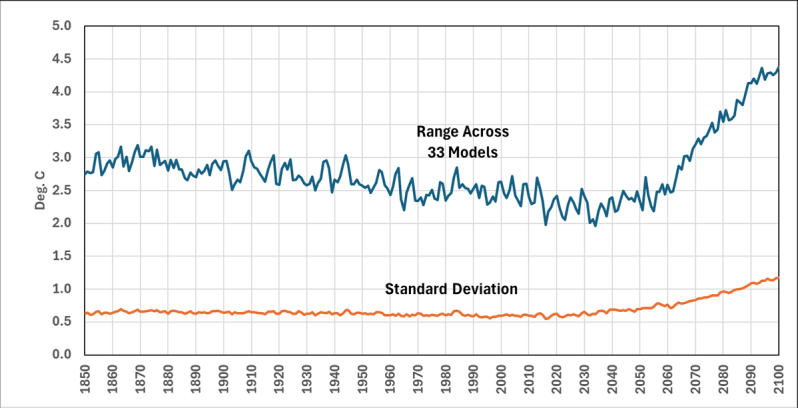
\includegraphics[width=.9\textwidth]{bilder/bilderKlima-0024.png}
  \captionof{figure}{CMIP6 Durchschnittliche Oberflächentemperaturspanne über 33 Modelle und Standardabweichung unter Verwendung des SSP5-85-Szenarios. Daten: KNMI Climate Explorer (\url{https://climexp.knmi.nl/start.cgi}).}
\end{minipage}

Jenseits der Fähigkeit der Modelle, Merkmale des heutigen Klimas zu reproduzieren, ist die kritische Frage für die Gesellschaft, wie gut sie Reaktionen auf subtile menschliche Einflüsse vorhersagen, wie Treibhausgasemissionen, Aerosol-Abkühlung und Landnutzungsänderungen. Der wichtigste Aspekt, den Modelle korrekt erfassen müssen, sind "Rückkopplungen". Diese treten auf, wenn Klimaänderungen entweder weitere Erwärmung verstärken oder unterdrücken. Im Allgemeinen verdoppelt oder verdreifacht der modellierte Nettoeffekt aller Rückkopplungen die direkte Erwärmungswirkung von CO$_2$.
\end{fullbox}

\section{Oberflächenerwärmung}
Ein einfacher Test der Gültigkeit eines Klimamodells ist seine Fähigkeit, historische Erwärmung als Reaktion auf bekannte vergangene Änderungen in Klimaantrieben wie Treibhausgasen zu reproduzieren. Abbildung 5.2 ist aus Scaffeta (2023) reproduziert, die die neueste Generation (CMIP6) von Klimamodellen in niedrige ECS ($1.5$ bis \SI{3.0}{\celsius}), mittlere ECS ($3.0$ bis \SI{4.5}{\celsius}) und hohe ECS ($4.5$ bis \SI{6.0}{\celsius}) gruppiert und ihre Post-1980 globalen Durchschnittstemperatur-Simulationsbereiche mit denen von drei Oberflächentemperaturaufzeichnungen und einem satelliten-basierten unteren Troposphärentemperatur-Datenprodukt vergleicht.
Die linke Spalte zeigt, dass die niedrig-ECS-Modelle die Post-1980 historische Erwärmungsaufzeichnung vernünftig gut verfolgen, aber die mittleren und rechten Spalten zeigen, dass die mittleren und hohen ECS-Modelle die Erwärmung auffällig über-vorhersagen.

\begin{figure}[H]
\begin{center}
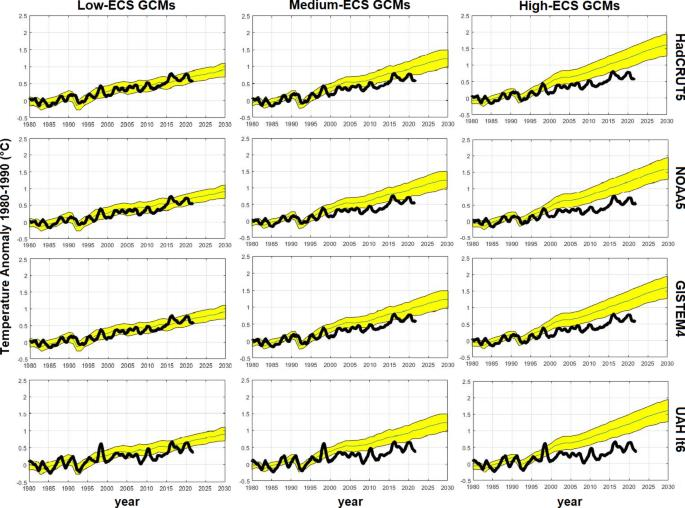
\includegraphics[width=1.0\textwidth]{bilder/bilderKlima-0026.jpg}\\[1cm]
\end{center}
\caption{Modell-Beobachtungs-Vergleiche für die Erwärmung der Erdoberfläche. Die Spalten entsprechen
Modellgruppen mit niedrigem ECS (13 Modelle), mittlerem ECS (11 Modelle) und hohem ECS (14 Modelle),
während die Zeilen den weit verbreiteten beobachteten Temperaturaufzeichnungen entsprechen, wobei die ersten drei
Oberflächendurchschnitte und die vierte den Durchschnitt der unteren Troposphäre zeigen. In jedem Feld bezeichnet der gelbe
Bereich den Mittelwert und die Spannweite (± eine Standardabweichung) der Klimamodellsimulationen für diese
Gruppe. Die dicke schwarze Linie zeigt die beobachtete jährliche Durchschnittstemperatur in der angegebenen Aufzeichnung.
Quelle: Scafetta (2023) Abb. 2.}
\end{figure}

Spencer (2024) hat auch eine nützliche Zusammenfassung der Modell-Beobachtungs-Diskrepanz bereitgestellt, indem er Trends in Oberflächentemperatur-Datenprodukten mit denen in einzelnen Klimamodellen verglich, wie in Abbildung 5.3 zusammengefasst; die meisten Klimamodelle zeigen erheblich mehr Erwärmung als die Beobachtungen seit 1979.

\begin{figure}[H]
\begin{center}
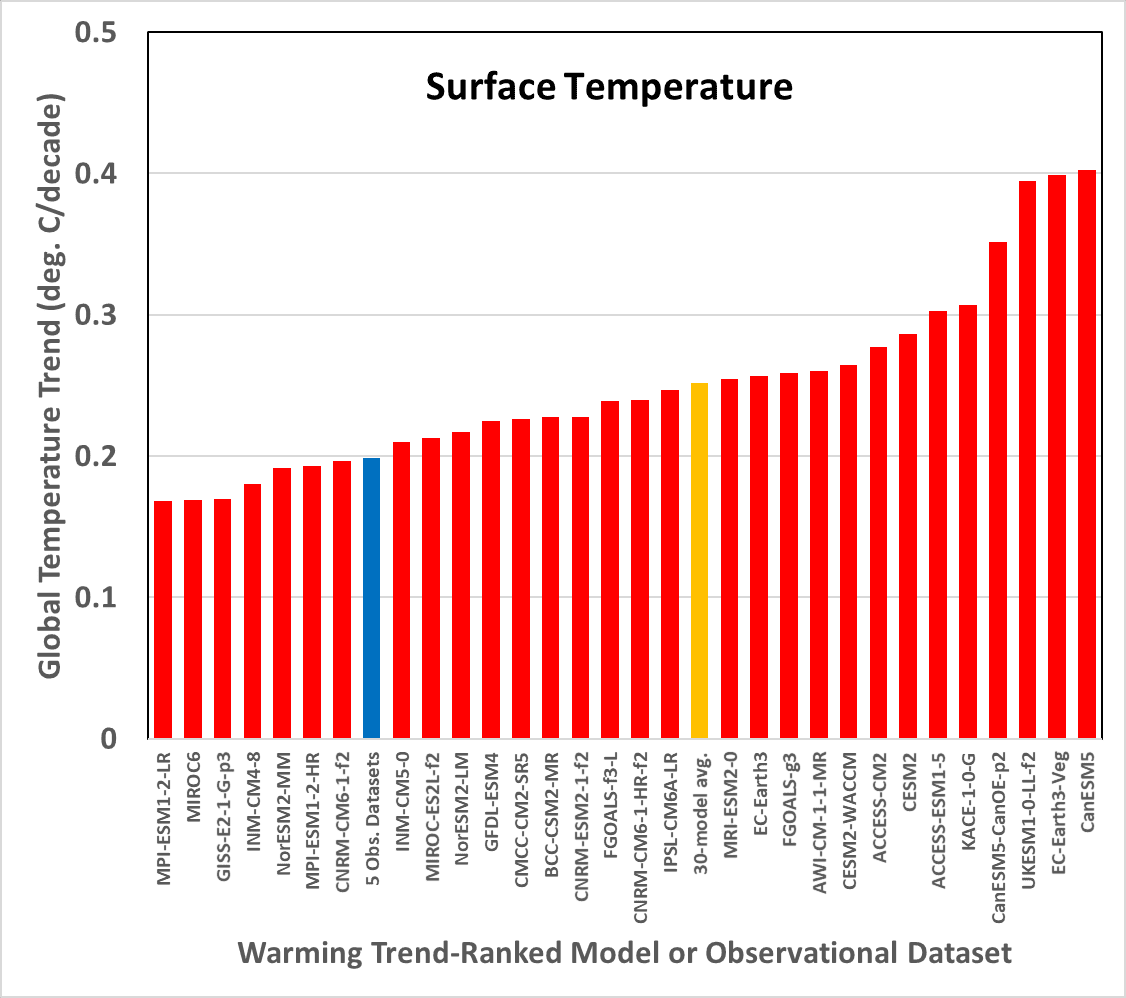
\includegraphics[width=1.0\textwidth]{bilder/bilderKlima-0027.png}\\[1cm]
\end{center}
\caption{Globale Trends der Oberflächenlufttemperatur (°C/Jahrzehnt), 1979–2024, aus verschiedenen CMIP6-Klimamodellen
(rot, Durchschnitt von 30 Modellen in orange); und der Durchschnitt von drei Thermometer-Datensätzen
(HadCRUT5, NOAA Global Temp und Berkeley 1 deg.) und zwei Reanalyse-Datensätzen (ERA5 und
NCEP/NCAR R1) in blau. Datenquelle: https://climexp.knmi.nl/start.cgi.}
\end{figure}

\section{Troposphärische Erwärmung}
Es ist seit langem bekannt, dass Klimamodelle im Durchschnitt die Erwärmung in der tropischen Troposphäre übertreiben. Diese Region ist ein wichtiger Test für Klimamodelle, da hier das Signal anthropogener Treibhauserwärmung zuerst und am stärksten auftritt. Verzerrungen in troposphärischen Trends zeigen Modellfehler in Wärmeübertragungsprozessen an, die sich auf Oberflächenerwärmungsverzerrungen übertragen.

Die Diskrepanz wurde als ernste Inkonsistenz im ersten U.S. Climate Change Science Program-Bericht (Karl et al. 2006) markiert und wurde in jedem IPCC-Bericht seitdem erwähnt, aber die Diskrepanz hat sich mit der Zeit verschlechtert, und die Verzerrung ist nun global. McKitrick und Christy (2020) verglichen troposphärische Erwärmungstrends in CMIP6-Klimamodellen mit beobachteten Trends von Satelliten, Wetterballons und Reanalysesystemen. Jedes Modell überschätzte den durchschnittlichen beobachteten Erwärmungstrend über 1979-2014 sowohl in unteren als auch mittleren Troposphärenschichten, sowohl global als auch in den Tropen. In den meisten einzelnen Modellen war die Verzerrung statistisch signifikant und im Durchschnitt über alle Modelle war sie hoch signifikant.

Abbildung 5.4 präsentiert die Vergleiche mit auf 2024 aktualisierten Daten (McKitrick und Christy 2025). Die jüngsten warmen Jahre bewegten den beobachteten Trend leicht nach oben und erweiterten die Trend-Konfidenzintervalle, aber das Gesamtmuster bleibt das gleiche: Modellverzerrung tendiert zu zu viel Erwärmung, in den meisten Fällen ist der Unterschied statistisch signifikant und im Durchschnitt ist die Verzerrung statistisch hoch signifikant. McKitrick und Christy (2020) zeigten auch, dass die Verzerrung in Modellen mit hoher ECS größer ist, aber selbst die Modelle mit niedrigerer durchschnittlicher ECS sagen zu viel Erwärmung vorher. Wenn zukünftige Klimamodelle globale troposphärische Erwärmung realistisch repräsentieren würden, wären sie wahrscheinlich weniger sensitiv als selbst die niedrig-ECS-Mitglieder des CMIP6-Ensembles.

\begin{figure}[H]
\begin{center}
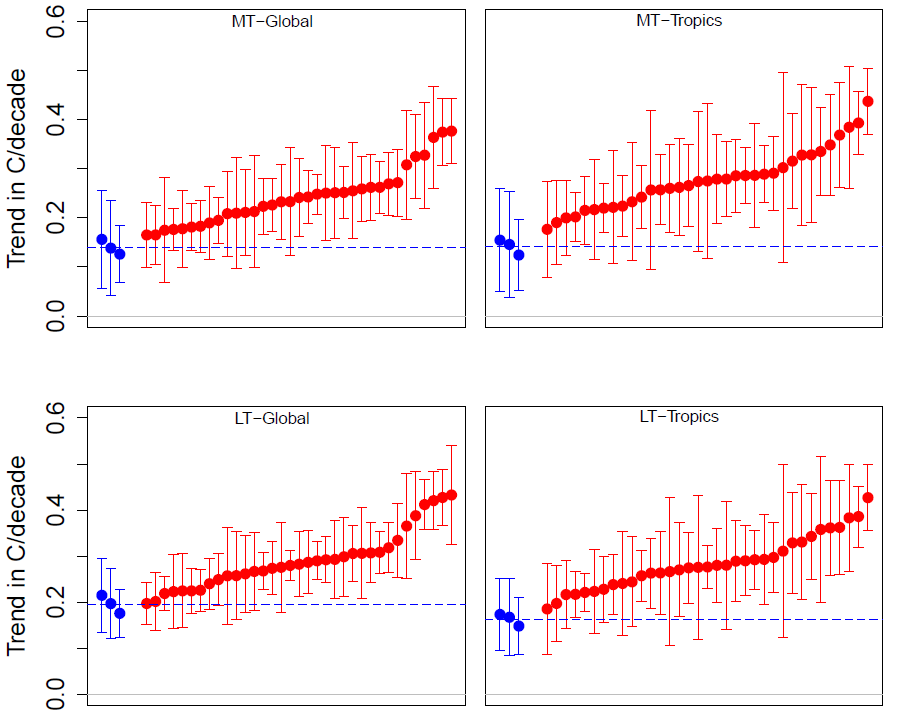
\includegraphics[width=1.0\textwidth]{bilder/bilderKlima-0028.png}\\[1cm]
\end{center}
\caption{Beobachtete gegenüber CMIP6-modellierten Erwärmungstrends (°C/Jahrzehnt 1979–2024) in der globalen
und tropischen unteren (LT) und mittleren Troposphäre (MT) unter Verwendung der Methodik von McKitrick und Christy
(2020) auf der Grundlage von Daten, die von 2014 bis 2024 aktualisiert wurden. Blaue Punkte: Erwärmungstrends mit 95-prozentigen Konfidenzintervallen
für 3 Datenprodukte (Radiosonden, Reanalyse und Satelliten). Blaue gestrichelte Linie: Durchschnittlicher Erwärmungstrend
für 3 beobachtete Reihen. Rote Punkte: Modellierte Erwärmungstrends mit 95-prozentigen Konfidenzintervallen
in 35 Modellen, angeordnet vom niedrigsten zum höchsten Wert.}
\end{figure}


Wie zuvor erwähnt, hat das IPCC die Modell-Beobachtungs-Diskrepanz lange anerkannt. Zum Beispiel bietet AR6 S. 443-444 dies zur tropischen Troposphäre (es behandelt nicht den globalen Vergleich):


\begin{quote}
Mehrere Studien seit AR5 haben weiterhin eine Inkonsistenz zwischen simulierten und beobachteten Temperaturtrends in der tropischen Troposphäre demonstriert, wobei Modelle mehr Erwärmung simulieren als Beobachtungen (Mitchell et al., 2013, 2020; Santer et al., 2017a, b; McKitrick und Christy, 2018; Po-Chedley et al., 2021)... Über den Zeitraum 1979–2014 sind Modelle konsistenter mit Beobachtungen in der unteren Troposphäre und am wenigsten konsistent in der oberen Troposphäre um 200 hPa, wo Verzerrungen \SI{0.1}{\celsius} pro Jahrzehnt überschreiten.
Mehrere Studien mit CMIP6-Modellen legen nahe, dass Unterschiede in der Klimasensitivität ein wichtiger Faktor sein könnten, der zur Diskrepanz zwischen simulierten und beobachteten troposphärischen Temperaturtrends beiträgt (McKitrick und Christy, 2020; Po-Chedley et al., 2021), obwohl es schwierig ist, den Einfluss von Klimasensitivität, Änderungen in Aerosolforcing und interner Variabilität bei der Beitragung zu troposphärischen Erwärmungsverzerrungen zu entschlüsseln (Po-Chedley et al., 2021). Eine andere Studie fand, dass das Fehlen einer hypothetischen negativen tropischen Wolkenrückkopplung die Hälfte der oberen Troposphären-Erwärmungsverzerrung in einem Modell erklären könnte (Mauritsen und Stevens, 2015).

... Zusammenfassend finden Studien weiterhin, dass CMIP5- und CMIP6-Modell\-simulationen mehr erwärmen als Beobachtungen in der tropischen mittleren und oberen Troposphäre über den Zeitraum 1979–2014 (Mitchell et al., 2013, 2020; Santer et al., 2017a, b; Suárez-Gutiérrez et al., 2017; McKitrick und Christy, 2018), und dass überschätzte Oberflächenerwärmung teilweise verantwortlich ist (Mitchell et al., 2013; Po-Chedley et al., 2021). ... Daher bewerten wir mit mittlerem Vertrauen, dass CMIP5- und CMIP6-Modelle weiterhin beobachtete Erwärmung in der oberen tropischen Troposphäre über den Zeitraum 1979–2014 um mindestens \SI{0.1}{\celsius} pro Jahrzehnt überschätzen.
\end{quote}

Bemerkenswert ist, dass trotz der Anhäufung von Belegen für überschüssige Modellerwärmung das IPCC nur mittleres Vertrauen in die Existenz einer Erwärmungsverzerrung zuordnet.

% --- Literatur ---
% \begin{thebibliography}{9}
% \bibitem{key} Autor. \emph{Titel}. Verlag/Journal, Jahr.
% \end{thebibliography}

\end{document}